% VLDB template version of 2020-03-05 enhances the ACM template, version 1.7.0:
% https://www.acm.org/publications/proceedings-template
% The ACM Latex guide provides further information about the ACM template
\documentclass[sigconf, nonacm]{acmart}
%% The following content must be adapted for the final version
% paper-specific

\usepackage{color}
\usepackage{enumitem}
\usepackage{float}
\usepackage{balance}% for  \balance command ON LAST PAGE  (only there!)
\usepackage{algorithm, algorithmicx}
\usepackage[noend]{algpseudocode}
\usepackage{tabu}
\usepackage{balance}
\usepackage{booktabs}
\usepackage{graphicx}
\usepackage{subfigure}
%\usepackage{times}
\usepackage{stfloats}
\usepackage{url}
\usepackage{comment}
\usepackage{amsmath}
\usepackage{makecell}
\usepackage{xcolor}
\usepackage{flushend}

\newcommand\vldbdoi{XX.XX/XXX.XX}
\newcommand\vldbpages{XXX-XXX}
% issue-specific
\newcommand\vldbvolume{14}
\newcommand\vldbissue{1}
\newcommand\vldbyear{2020}
% should be fine as it is
\newcommand\vldbauthors{\authors}
\newcommand\vldbtitle{\shorttitle}

%
\newtheorem{problem}{Problem}
\newtheorem{lemma}{Lemma}
\newtheorem{theorem}{Theorem}
\newcommand{\Bo}[1]{{\color{red} Bo: #1}}

\newcommand{\QM}[1]{{\color{blue}{#1}}}
\newcommand{\REPORT}[1]{{\color{purple}{#1}}}

\newcommand{\D}{\mathcal{T}}
\newcommand{\V}{\mathsf{V}}
\newcommand{\oR}{\mathcal{R}}
\newcommand{\MU}{\mathsf{U}}
\newcommand{\vats}{\mathsf{VFGS}}
\newcommand{\rand}{\mathsf{RAND}}
\newcommand{\full}{\mathsf{FULL}}
\newcommand{\avats}{\mathsf{VFGS}^{+}}
\newcommand{\cavats}{\mathsf{VFGS}^{+}\mathsf{CE}}
\newcommand{\sz}{\textsf{Shenzhen}}
\newcommand{\pt}{\textsf{Porto}}
\newcommand{\trim}{\vspace{-2mm}}

\newcommand{\stitle}[1]{\vspace*{0.4em}\noindent{\bf #1:\/}}
\newcommand{\sstitle}[1]{\vspace*{0.4em}\noindent{\bf #1\/.}}


\newcommand{\squishlist}{
 \begin{list}{$\bullet$}
 { \setlength{\itemsep}{0pt}
   \setlength{\parsep}{3pt}
   \setlength{\topsep}{3pt}
   \setlength{\partopsep}{0pt}
   \setlength{\leftmargin}{1.2em}
   \setlength{\labelwidth}{1em}
   \setlength{\labelsep}{0.6em}
 }
}
\newcommand{\squishend}{
 \end{list}
}

\settopmatter{printfolios=true}



\begin{document}
\title{Visual Fidelity-Guaranteed Sampling for \\ Large-scale Trajectory Data Visualization}

%\author{Qiaomu Shen$^{*}$,\quad Chuan Yang$^{*}$,\quad Chaozu Zhang$^{*}$,\quad Dan Zeng$^{\dag}$, \quad Wei Zeng$^{\ddag}$, \quad Bo Tang$^{*}$}

\affiliation{
  \institution{Qiaomu Shen$^{\dag}$,\quad Chaozu Zhang$^{\dag}$,\quad Chuan Yang$^{\dag}$, \quad Xiao Yan$^{\dag}$, \quad Dan Zeng$^{\ddag}$, \quad Wei Zeng$^{\$}$, \quad Bo Tang$^{\dag}$}
  \institution{$^{\dag}$ Department of Computer Science and Engineering, Southern University of Science and Technology}
  \mbox{qshen@connect.ust.hk, \{11612732@mail,11712021@mail, tangb3@\}sustech.edu.cn} \\
  \institution{$^{\ddag}$ Electrical Engineering, Mathematics and Computer Science, University of Twente}
  \institution{$^{\$}$ Shenzhen Institutes of Advanced Technology, Chinese Academy of Sciences}
  \mbox{xyan@cse.cuhk.edu.hk, d.zeng@utwente.nl, zengwei81@gmail.com}
  %\email{{{11711004, 11712532, 11613015}@mail.,tangb3@}sustech.edu.cn}
  %\mbox{qshen@connect.ust.hk, \{11612732@mail,11712021@mail,tangb3@\}sustech.edu.cn, d.zeng@utwente.nl, zengwei81@gmail.com}
}

\renewcommand{\shortauthors}{Qiaomu Shen, et al.}
\renewcommand{\shorttitle}{Paper ID: 324}

%% The abstract is a short summary of the work to be presented in the
%% article.
\begin{abstract}
Visualizing large-scale trajectory data is a core subroutine for many smart city applications, e.g., traffic management, urban planning, and route recommendation. The task is challenging due to high scalability requirement and severe visual clutter. Sampling can effectively mitigate both problems but may harm visual fidelity, i.e., generating visualizations that look different from the exact one. In this work, we propose sampling techniques that provide \textit{theoretically guaranteed visual fidelity} for large-scale trajectory data visualization. We first define a natural pixel-based \textit{fidelity loss function} to measure the difference between two visualizations. However, our analysis shows that it is NP-hard to sample a fixed-size subset of trajectories to minimize the loss function. Therefore, we then devise an approximate algorithm named \textit{$\vats$} with a suite of optimization techniques, which runs efficiently but still provides guaranteed fidelity loss. By taking data distribution and human perception characteristics into consideration, we further improve $\vats$ to an advanced algorithm named $\avats$ to tackle the visual clutter problem. Extensive experiments (i.e., case-, user-, and quantitative- studies) are also conducted on real-world trajectory datasets to verify the effectiveness and efficiency of our proposals.
%In addition, comprehensive user studies further illustrate the superiority of our proposals in various applications, e.g., traffic flow comparison, and reachable route inspection.
\end{abstract}

\maketitle

\trim \trim

\begingroup\small\noindent\raggedright\textbf{PVLDB Reference Format:}\\
\shortauthors. Visual Fidelity-Guaranteed Sampling for Large-scale Trajectory Data Visualization. PVLDB, \vldbvolume(\vldbissue): \vldbpages, \vldbyear.\\
\href{https://doi.org/\vldbdoi}{doi:\vldbdoi}
\endgroup

\trim \trim %\trim

\begingroup
\renewcommand\thefootnote{}\footnote{\noindent
This work is licensed under the Creative Commons BY-NC-ND 4.0 International License. Visit \url{https://creativecommons.org/licenses/by-nc-nd/4.0/} to view a copy of this license. For any use beyond those covered by this license, obtain permission by emailing \href{mailto:info@vldb.org}{info@vldb.org}. Copyright is held by the owner/author(s). Publication rights licensed to the VLDB Endowment. \\
\raggedright Proceedings of the VLDB Endowment, Vol. \vldbvolume, No. \vldbissue\ %
ISSN 2150-8097. \\
\href{https://doi.org/\vldbdoi}{doi:\vldbdoi} \\
}\addtocounter{footnote}{-1}\endgroup
%%% VLDB block end %%%

\section{Introduction}\label{sec:intro}
Nowadays, the ubiquity of location-acquisition devices leads to an explosive growth of the volume of movement data (i.e., trajectories), e.g., for vehicles, shared bikes and pedestrians. Visualizing these large-scale trajectory data is crucial for many smart city applications~\cite{wang2014visual,tang2017efficient,zheng2011learning} and location-based services~\cite{liu2016smartadp, zheng2010collaborative}. Among various visualization methods, line-based trajectory visualization, which connects the locations of a moving object by polylines, is widely adopted for spatial-temporal data analytics~\cite{chen2015survey,visualanalysis,bigchanvis}. However, large-scale line-based trajectory visualization suffers from two problems--(i) \textit{scalability} and (ii) \textit{visual clutter}, which we elaborate as follows.


%\stitle{Large trajectory data size and limited rendering capability of graphics device}
\stitle{Scalability}
Trajectory datasets can be extremely large and thus take a long time to render for visualization. For example, Shenzhen has 24,237 taxis which collectively generate more than 82.8 million GPS locations each day~\cite{sz}. Our benchmark on the \pt{} taxi trajectory dataset shows that it takes 13.95 seconds to render 1 million real-world trajectories using an NVIDIA GeForce GTX 1080 GPU with 8GB video memory. The long delay caused by large dataset cardinality makes interactive visual exploration difficult. Thus, we want visualization to scale to very large datasets while maintaining a short delay.

%In New York, {there are} over 13,000 taxis carrying over 1 million passengers and making 500,000 trips on an average day~\cite{ferreira2013visual}.

%Rendering refers to the use of the hardware device (e.g., GPU) in the generation of visualizations.

%However, the rendering capability of modern commodity GPUs is limited.
%We did a benchmark experiment to evaluate the rendering capability of NVIDIA GeForce GTX 1080 with 8GB video memory.
%It needs 13.95 seconds to render 1 million real-world trajectories in \pt{}. % with 32.66 millions GPS points.
%Obviously, it cannot support interactive visual exploration in large-scale trajectory dataset.
%Thus, how to support scalable visualization is the first challenge in large trajectory data visualization problem.

\stitle{Visual clutter} It is a common problem for large-scale data visualization~\cite{clutter}, which we illustrate with an example in Figure~\ref{fig:teaser}(A). Because of visual clutter, it is almost impossible to recognize the road network in the embedded figure of Figure~\ref{fig:teaser}(A), making it difficult for human-users to gain insights from the visualization. Hence, we want the trajectory visualization to be visual-clutter-free for good user experience.

%It is almost impossible to
%
%It is a common issue in big data visualization~\cite{clutter}.
%Figure~\ref{fig:teaser}(A) is the visualization result of the full \pt{} taxi trajectory dataset.
%Intuitively, the region shown in the embedded figure of A suffers visual clutter issue seriously,
%i.e., the road network almost cannot be recognized in it,
%which hinders the abilities of human-users to explore the dataset and identify the underlying data insights.
%Hence, the second challenge in large trajectory data visualization problem is how to address visual clutter issue.



%To overcome the above challenges, several visualization approaches have been proposed in the literature.
%Unfortunately, none of them could address these three challenges simultaneously and perfectly.
%In particular, the spatial aggregation based approaches~\cite{zeng2013visualizing,von2015mobilitygraphs} preprocess the massive movement data, and visualize the results after preprocessing.
%The aggregation based methods ignored the visual clutter in raw spatial data as they only visualize the aggregated/preprocessed results.
%In other words, their visualization results may lose the detail information in raw data.
%%These approaches alleviate the large data size and limited rendering ability issues in large-scale spatial data visualization.
%%Nevertheless, they ignored the visual clutter issue in raw spatial data as they only visualize the aggregated/preprocessed results.
%In recent years, many visualization research works are proposed to address visual clutter,
%e.g., edge bundling~\cite{zeng2019route, thony2015vector} and density map~\cite{lampe2011interactive, scheepens2011interactive}.
%However, these works neither focus on line-based trajectory visualization nor designed for large-scale trajectory dataset.

\begin{figure*}[t]
	\centering
	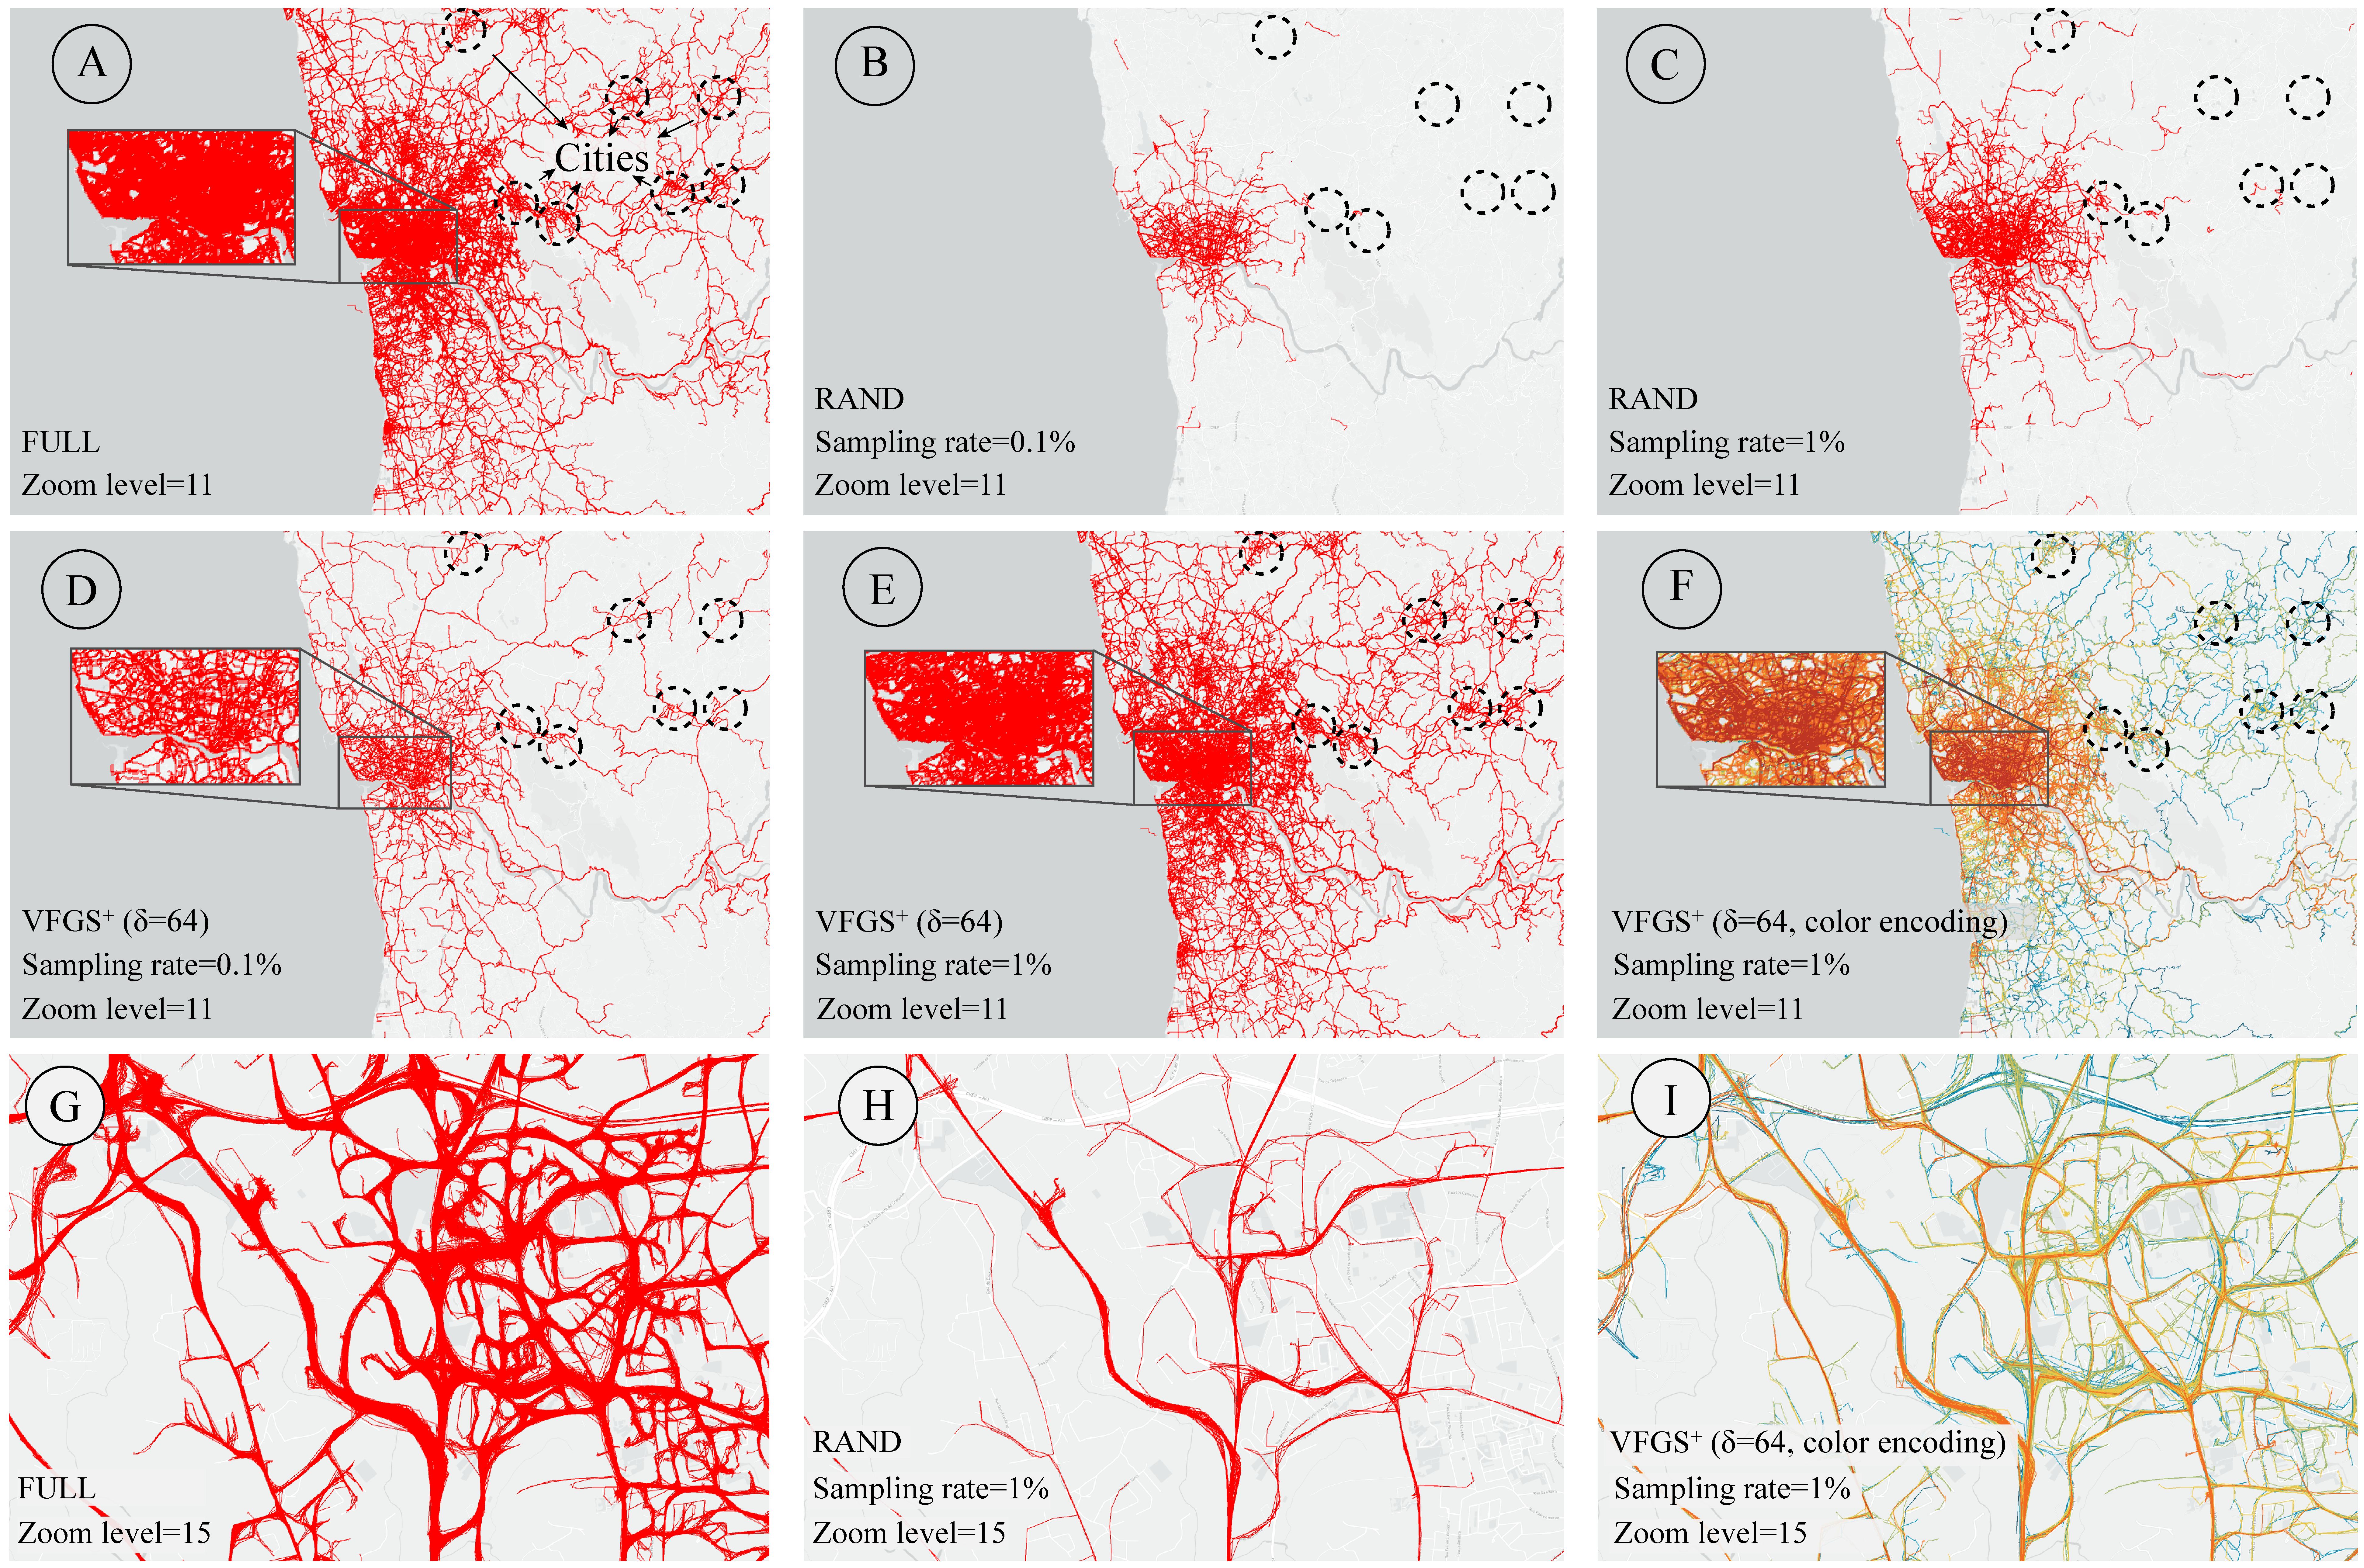
\includegraphics[width=0.85\textwidth]{pictures/Teaser.pdf}
	\vspace{-3mm}
	\caption{A comparison of visualization results. (I) A is the visualization of the full \pt{} taxi trajectory dataset at zoom level 11.
    At the same zoom level, B and C are produced by uniform random sampling,
    while D, E, F are produced by our $\avats$ algorithm.
    (II) G is the visualization of the full \pt{} dataset at zoom level 15, while H and I are the corresponding results of uniform random sampling and $\avats$, respectively.
    (III) F and I are generated by $\avats$ with color encoding for representativeness to combat visual clutter.
    Best viewed in color.}
	\label{fig:teaser}
\trim
\end{figure*}

Sampling techniques are widely used for large-scale data analysis in both database and visualization communities~\cite{qin2020making,DBLP:conf/sigmod/DingHCC016,DBLP:journals/pvldb/KimBPIMR15,park2016visualization}. By sampling a subset of records from the raw large-scale dataset, it helps to reduce the rendering latency on graphics devices for visualization. One such example is ScalaR~\cite{battle2013dynamic}, which employs a reduction layer between the visualization layer and the data management layer. The reduction layer samples records \textit{uniformly at random} (denoted as $\rand$) when the query results are too large. However, $\rand$ does not work well for large-scale trajectory data visualization as it cannot provide fidelity guarantee. Take Figure~\ref{fig:teaser}(B) and (C) for example, they are the visualization results generated by $\rand$ on the \pt{} taxi trajectory dataset with sampling rate $0.1\%$ and $1\%$, respectively. Obviously, both of them are very different from the visualization of the full \pt{} dataset in Figure~\ref{fig:teaser}(A).


%In general, it samples a subset of data from the raw large-scale dataset, then it could be rendered efficiently by the graphics device.
%For example, ScalaR~\cite{battle2013dynamic} employs a reduction layer between the visualization layer and the data management layer.
%The reduction layer embedded a uniform random sampling algorithm to sample data randomly when the query results are large enough.
%It then reduces the amount of data to be visualized.
%However, the uniform random sampling method does not work well in the large trajectory data visualization problem as it does not provide guarantees about the sampling results.
%Take Figure~\ref{fig:teaser}(B) and (C) as examples,
%they are the visualization results of uniform random sampling method $\rand$ on \pt{} taxi trajectory dataset with sampling rate $0.1\%$ and $1\%$, respectively.
%Visually, both visualized results cannot capture the overview of the \pt{} trajectory dataset in Figure~\ref{fig:teaser}(A).

In this work, we set out to design efficient sampling algorithms that provides visual fidelity guarantee for line-based large-scale trajectory visualization. This goal leads to three research problems: (i) \emph{how to measure the visual fidelity of one visualization result?} (ii) \emph{how to devise an efficient sampling algorithm that provides  guaranteed visual fidelity?} (iii) \emph{how to tackle the visual clutter problem in large trajectory visualization?} To address these problems, we first propose a novel pixel-based \textit{visual fidelity loss function} to formally measure the difference between two visualizations. We then show that it is NP-hard to select a sized-$k$ sample of the trajectories to minimize the visual fidelity loss function. Next, we devise an \textit{efficient approximate algorithm }named $\vats$, which provides theoretical visual fidelity guarantee for the sampled results. Last, we \textit{explicitly tackle the visual clutter problem} by taking data distribution and human perception characteristics into consideration in an advance algorithm named $\avats$.

%In this work, we propose visual fidelity-guaranteed sampling approaches for the line-based trajectory visualization problem.
%The technical challenges of our proposal are
%(i) \emph{how to define visual fidelity of visualization result theoretically?}
%(ii) \emph{how to devise an efficient sampling algorithm which offers visual fidelity guarantee on the visualization result?}
%and (iii) \emph{how to overcome the visual clutter in large trajectory visualization?}
%Specifically, we first propose a novel pixel-based visual fidelity loss function between two visualization results formally.
%With the visual fidelity loss function, we then prove it is NP-hardness to select a sized-$k$ subset of trajectories which has the minimal visual fidelity loss.
%Next, we devise an approximate algorithm $\vats$ which returns a sized-$k$ subset of trajectories and offers theoretical visual fidelity guarantee on the returning result.
%Last, we address the visual clutter issue explicitly by taking data distribution and human perception capability into consideration in the advance approach $\avats$.

We illustrates the merits of our proposals in Figure~\ref{fig:teaser}. Figure~\ref{fig:teaser}(D) and (E) are the results of our $\avats{}$ algorithm on the \pt{} dataset with sampling rate $0.1\%$ and $1\%$, respectively. Compared with their uniform random sampling (i.e., $\rand$) counterparts Figure~\ref{fig:teaser}(B) and (C), they are obviously more similar to the full dataset visualization in Figure~\ref{fig:teaser}(A). The advantage of our proposals over $\rand$ is also consistent across different zoom levels, e.g., Figure~\ref{fig:teaser}(E) vs. Figure~\ref{fig:teaser}(C) at level 11, and Figure~\ref{fig:teaser}(I) vs. Figure~\ref{fig:teaser}(H) at level 15. Figure~\ref{fig:teaser}(F) is produced by our $\avats{}$ algorithm using the same parameters as Figure~\ref{fig:teaser}(E) but the trajectories are colored according to their algorithm-generated representativeness (warmer color means more representative). Observe that the visual clutter problem in Figures~\ref{fig:teaser}(A) and (E) are significantly alleviated in Figure~\ref{fig:teaser}(F) with color encoding. This advantage is even more prominent when comparing Figure (I) with Figure (G) and (H).




%Figures~\ref{fig:teaser}(D) and (E) show the visualization results of our proposal $\avats{}$ on \pt{} taxi trajectory dataset with {the} sampling rate $0.1\%$ and $1\%$, respectively.
%Comparing with the corresponding visualization results of uniform random sampling method $\rand$ in Figure~\ref{fig:teaser}(B) and (C),
%the superiority of $\avats$ is obvious.
%% Obviously, the visualization fidelity of them are much better than the uniform random sampling visualization results with the same sampling rates, see Figure~\ref{fig:teaser}(B) and (C).
%Figures~\ref{fig:teaser}(F) is the returning result of our proposal, which colors the trajectories {according to the trajectory representativeness}.
%It has the same parameters of Figure~\ref{fig:teaser}(E).
%Visually, the visual clutter issue in Figures~\ref{fig:teaser}(A) and (E) are alleviated in Figure~\ref{fig:teaser}(F).
%In addition, our proposals are robustness with different zoom levels.
%%Figure~\ref{fig:teaser}(G), (H), and (I) depict the visualization results of the \pt{} dataset, the returning result of uniform random sampling $\rand$ and the returning result of $\avats$ with color encoding at zoom-level 15, for example, we can obtain them by zooming in the visualization result in Figure~\ref{fig:teaser}(A), (C), and (F), respectively.
%Consider the visualization results in Figures~\ref{fig:teaser}(G), (H), and (I) with zoom level 15.
%Intuitively, the visualization result of our proposal $\avats$ in Figure~\ref{fig:teaser}(F) outperforms the uniform random sampling $\rand$ in Figure~\ref{fig:teaser}(H) significantly.
%It even performs better than Figure~\ref{fig:teaser}(G), the visualized result of the \pt{} dataset, as it reduces visual clutter in Figure~\ref{fig:teaser}(G) by using color encoding scheme to capture the representativeness of different trajectories.

To sum up, our contributions in this paper include:
%\setlist{nolistsep}
%\begin{itemize}[noitemsep]
\squishlist
  \item We formulate the visual fidelity-guaranteed sampling problem for large-scale trajectory data visualization, and prove that it is {NP-hard} in Section~\ref{sec:pro}.
  \item We devise an approximate algorithm $\vats$ for the visual fidelity-guaranteed sampling problem with a suite of efficiency optimizations including submodularity and lazy computation in Section~\ref{sec:sol}.
  \item We propose an advance algorithm $\avats$ to tackle the visual clutter problem by introducing a perception tolerance parameter, and encoding the representativeness of trajectories using different colors in Section~\ref{sec:aa}.
  \item We conduct extensive experiments on real-world trajectory datasets to demonstrate the superiority of our proposals in Section~\ref{sec:exp}. In particular, nearly 200 real users are recruited to test the effectiveness of our methods on three practical applications.
\squishend
%\end{itemize}

% in Section~\ref{sec:pro}

%Our proposal demonstrates their superiority over existing methods
%With the same sampling set size($1\%$), the proposed method generates a higher-fidelity visualization and .

%With the loss function, we analyze the hardness of the problem, and devise a visual quality guaranteed sampling algorithm for it.
%Figure~\ref{fig:compare} depicts an comparison among the ground truth,  uniform random sampling and our proposed method.
%With the same sampling set size($1\%$), the proposed method generates a higher-fidelity visualization and support the multi-resolution very well.
%At last, color encoding are applied to enhance the distribution of trajectories.

%


%\TB{Visualizing a large collection of trajectories are used frequently in map service or smart city applications.}
%The most popular and conventional method is the line-based visualization~\cite{chen2015survey}: connecting the passing points of movement objects by polylines.
%To handle the big dataset, many visualization products such as Spotfire~\footnote{\url{https://www.tibco.com/products/tibco-spotfire}}
%and Tableau~\footnote{\url{https://www.tableau.com/}} support advanced database management systems as a ``backend'' for the efficient data processing the query.
%The current visualization tools always don't scale well for the presentation of very large trajectory dataset due to the two challenges,
%visual clutter and limited rendering speed, which hinders the abilities of human-users for interactively exploring the dataset and identifying the movement patterns.
%In recent years, most of the visualization research works mainly try to address the visual clutter issue by proposing new techniques such as the
%spatial aggregation~\cite{zeng2013visualizing, von2015mobilitygraphs}, edge bundling~\cite{zeng2019route, thony2015vector} and density map~\cite{lampe2011interactive, scheepens2011interactive}.
%Instead, in this paper, we focus on the challenge of inefficient rendering in the large trajectory dataset by involving data sampling techniques.

%It is time consuming to generate very simple visualization when the data size become very large. Using Porto taxi data ~\footnote{\url{http://www.geolink.pt/ecmlpkdd2015-challenge/dataset.html}} as an example, Table~\ref{table:rendering_time} demonstrates the rendering time at each dataset size. \ZW{shall also mention which rendering toolkit is used here.} It shows that normal method takes more than 14 minutes (\ZW{seconds?}) to generate the graphics for 1 million trajectories, which is far beyond the human-acceptable response time for the interactive exploration~\cite{shneiderman1984response}.
%One work closely related to ours is ScalaR~\cite{battle2013dynamic}, which adds a reduction layer between visualization layer and data management layer. The reduction layer uses an uniform random sampling method to sample data once the query results are large enough, thus to reduce the amount of data to be visualized.
%Further more, Park et al. propose VAS~\cite{park2016visualization} which implements new sampling techniques to guarantee the visual quality.
%However, these sampling techniques are designed for the simple dataset, and have been approved effective in scatter plot or map plot.
%However, the trajectory sampling is more challenge due to the complexity of data form(e.g. varying lengths, lack of compact representation, difficulty in measuring the similarity) that makes traditional density-biased sampling techniques inappropriate.
%A naive solution to employ sampling idea for large-scale trajectory visualization problem is randomly selecting several trajectories from the data set then visualize it by graphics device.
%However, the visualization result may be not acceptable by the user because of the visual information loss in the sparse distributed regions.





%
%\begin{figure}[t]
%	\centering
%	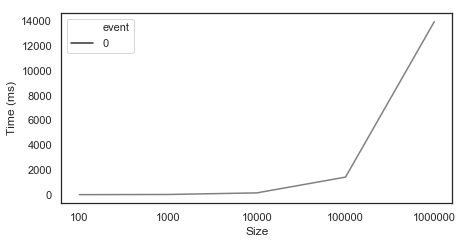
\includegraphics[width=0.4\textwidth]{pictures/introduction/timesize.png}
%	\vspace{-5mm}
%	\caption{The latency time for generating line-based visualization at each datasize.}
%	\vspace{-5mm}
%	\label{fig:rendering_time}
%\end{figure}




%The major challenges to design visual quality guaranteed sampling method are:
%(I) how to define visual quality theoretically? (II) how to guarantee the quality of the sampling-based visualization result?
%\TB{In this work, we study how to reduce the rendering time and preserve the visual quality for the large-scale trajectory visualization.}
%We extend the motivation of visualization-aware sampling to trajectory dataset and propose a novel sampling strategy, \textbf{v}isualization \textbf{a}ware \textbf{t}rajectory \textbf{s}ampling(VATS), that produces high-visual-quality line-based trajectory visualization at different zooming resolutions.
%%\QM{In this paper, we first proposed the visual fidelity loss function which effectively evaluates the visual loss of the sampling method. Then we minimize the loss function by transforming this problem to an optimization problem. Several solutions for efficiently solving the optimization problem are discussed.}
%We first format visual quality by defining the loss function between the visualization results of the whole dataset and sampled dataset.
%With the loss function, we analyze the hardness of the problem, and devise a visual quality guaranteed sampling algorithm for it.
%Figure~\ref{fig:compare} depicts an comparison among the ground truth,  uniform random sampling and our proposed method.
%With the same sampling set size($1\%$), the proposed method generates a higher-fidelity visualization and support the multi-resolution very well.
%At last, color encoding are applied to enhance the distribution of trajectories.
%
%\begin{figure}[t]
%	\centering
%	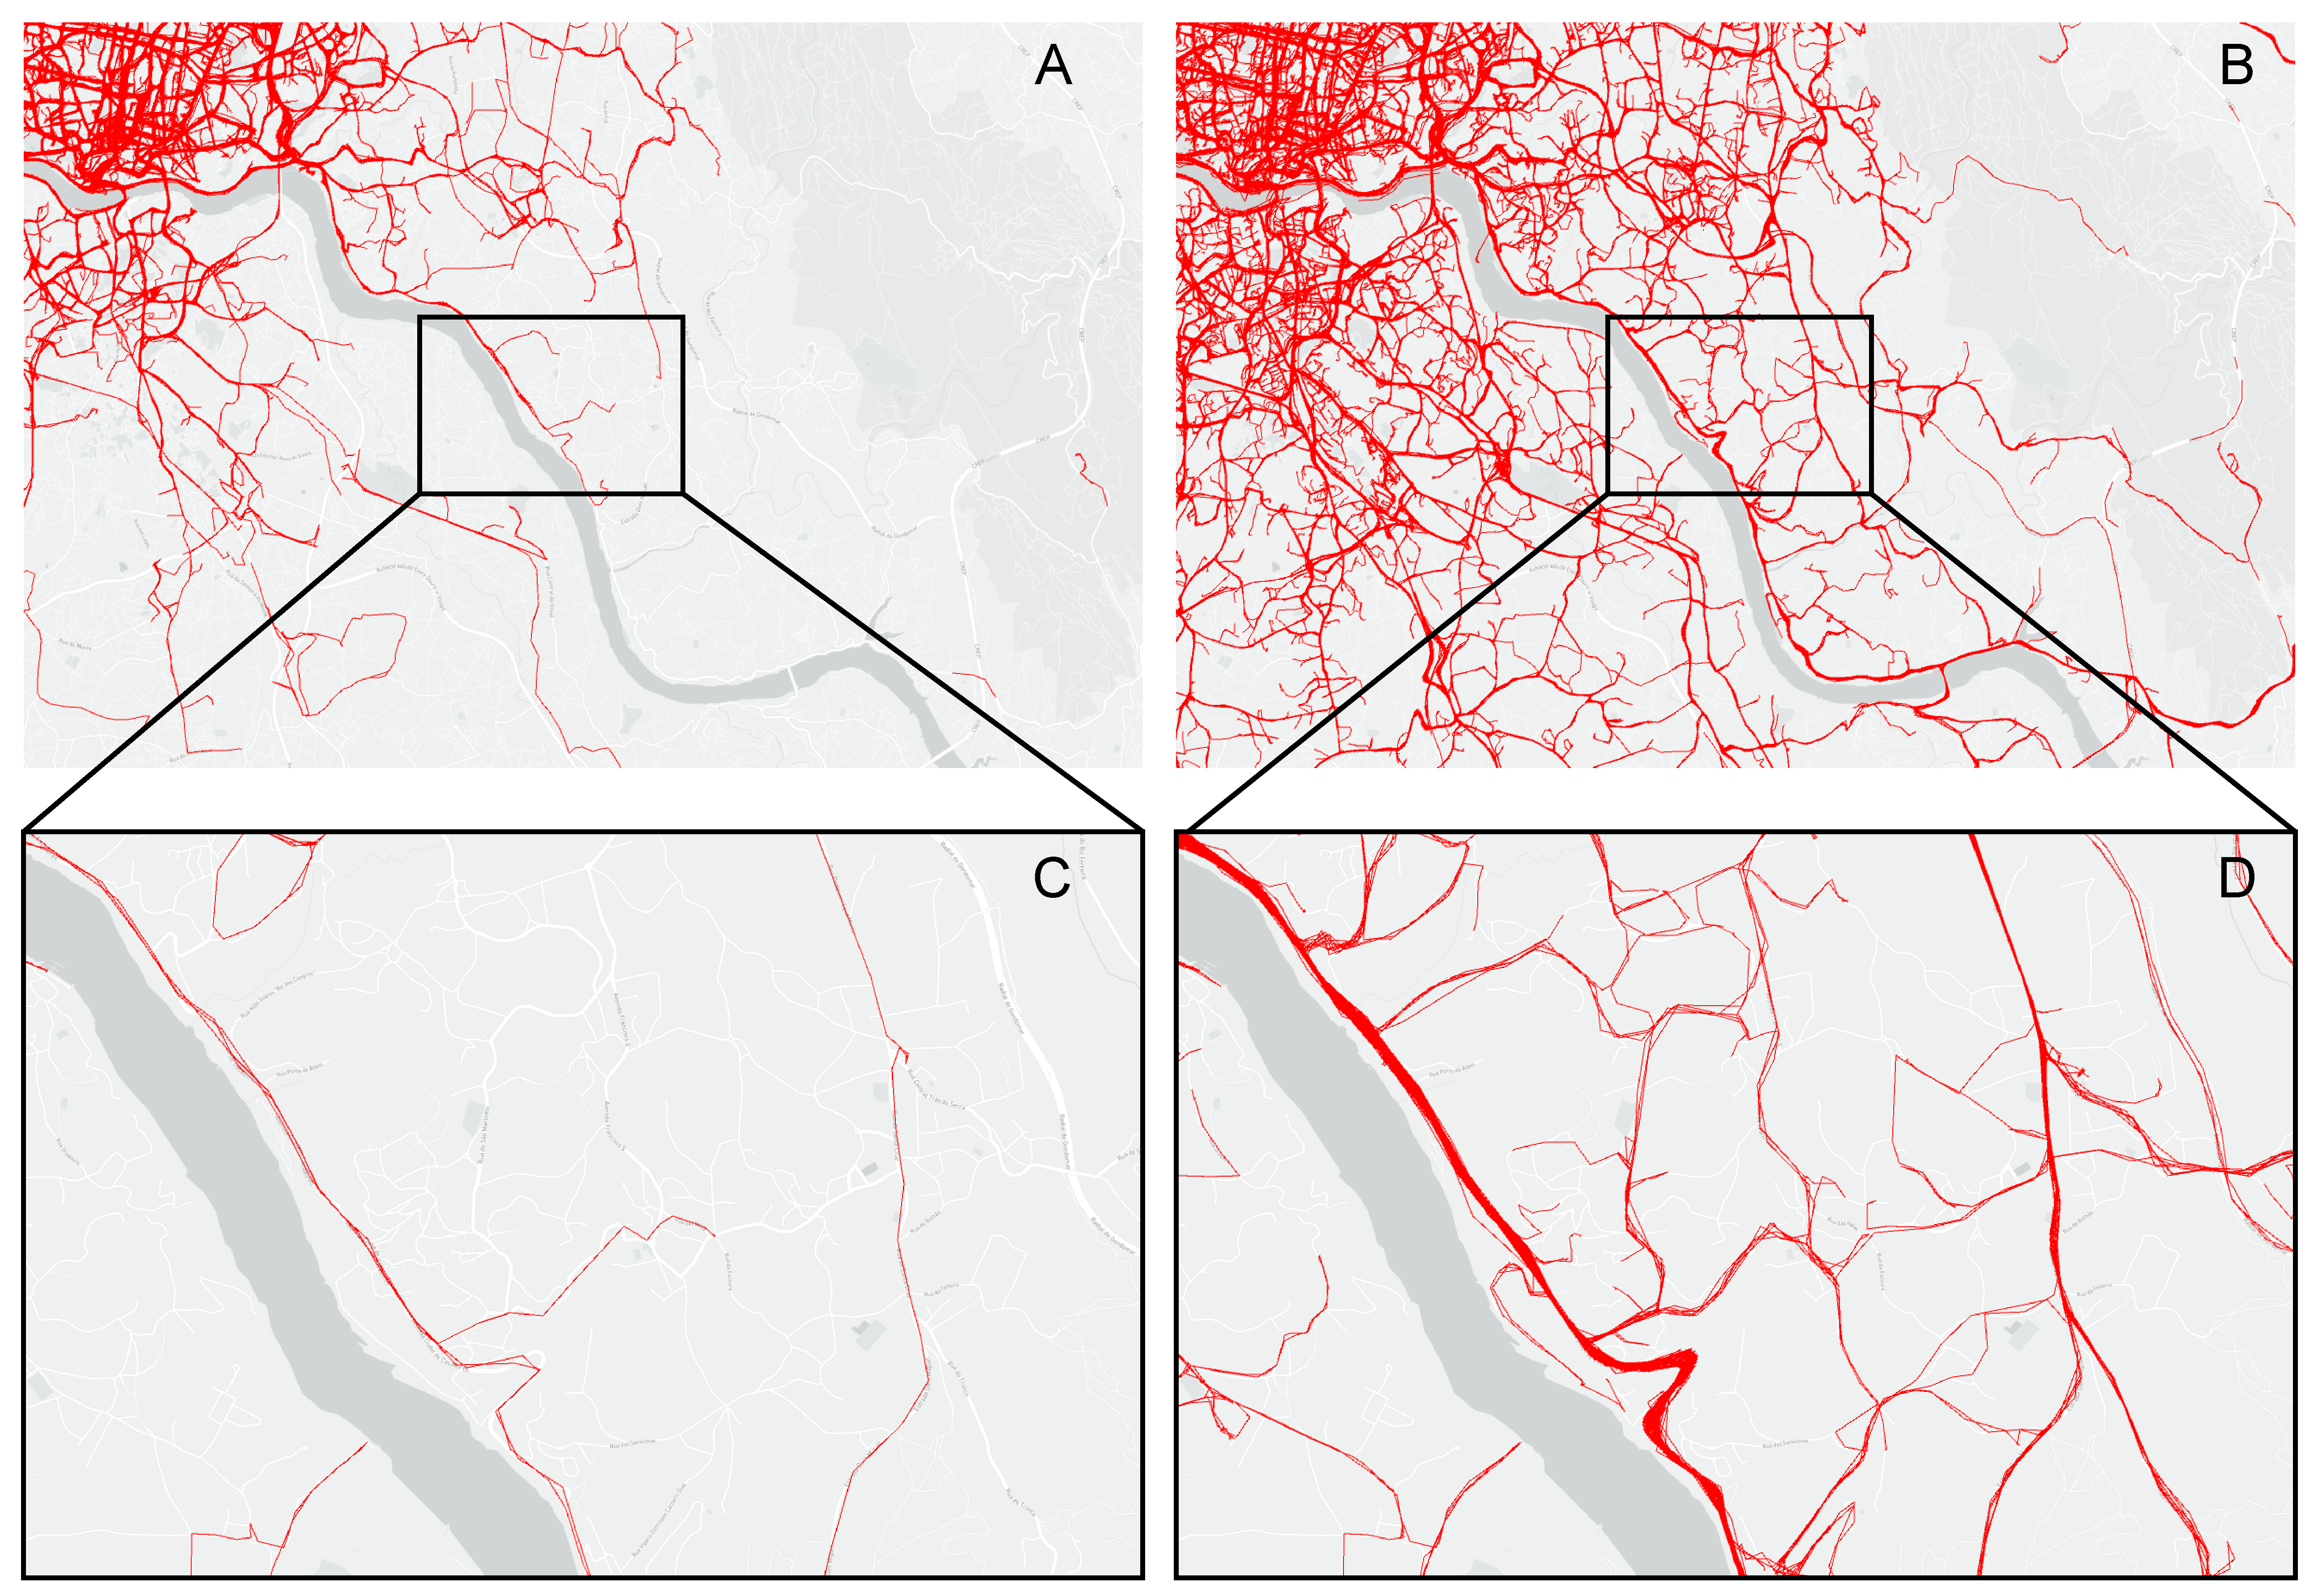
\includegraphics[width=0.44\textwidth]{pictures/introduction/effectiveness.pdf}
%	\vspace{-3mm}
%	\caption{Trajectory sampling generated by uniform random sampling(A,C) and VQGTS(B,D) at same sampling rate. In both high-level(A,B) and low level(C,D) view, our approach preserved more detail information about the trajectories especially for the sparse regions.}
%	\vspace{-5mm}
%	\label{fig:compare}
%\end{figure}
%

%
% \Bo{we can keep it at technical report.}
%The remainder of this paper is organized as follows. Section~\ref{sec:rel} discusses the related work, and Section~\ref{sec:pro} formally formulates our problem and analyze its hardness. Section~\ref{sec:sol} presents our approximate solution for the problem along with the optimization techniques. The advanced solution for visual clutter is introduced in Section~\ref{sec:aa}. Section~\ref{sec:exp} elaborates the extensive experimental studies. Section~\ref{sec:con} concludes this paper and highlights possible future directions.


%Section~\ref{sec:pro} formulates our problem and analyze its hardness.
%Section~\ref{sec:sol} provides an approximate solution for it, together with a suite of optimization techniques.
%Section~\ref{sec:aa} proposes an advanced solution for our problem.
%Section~\ref{sec:exp} elaborates our extensive experimental studies and our findings in detail.
%Section~\ref{sec:con} concludes this work and highlights the promising future directions.



\trim
\section{Related work}\label{sec:rel}
%In this section, we survey previous work and focus on the most relevant pieces.
%Section~\ref{sec:trajvisana} and ~\ref{sec:interactive} summarize the related works in trajectory visual analysis and interactive data visualization for large dataset, respectively.

In this part, we survey related works on \textit{trajectory visualization methods} in Section~\ref{sec:trajvisana} and \textit{interactive data visualization for large datasets} in Section~\ref{sec:interactive}, respectively.

\subsection{Trajectory Visualization Methods}\label{sec:trajvisana}
A trajectory is a sequence of spatial locations (e.g., GPS positioning results) and trajectory is the most common representation of object movements. Existing trajectory visualization methods can be classified into three categories according to the form of visualization~\cite{chen2015survey}, i.e., \textit{point-based visualization}, \textit{region-based visualization}, and \textit{line-based visualization}. We give a brief introduction to these methods and refer the interested readers to~\cite{chen2015survey} for more detailed discussions. Point-based visualization plots the locations in each trajectory independently and captures the overall spatial distribution of the moving objects. Many density-based methods, e.g., kernel density estimation, are applied in point-based visualization~\cite{liu2013vait,yang2016exploring,chae2014public,xie2008kernel, borruso2008network} to preserve the spatial distribution. Region-based visualization slices the entire region into sub-regions and visualizes the aggregated information in each sub-region~\cite{guo2009flow,wood2010visualisation,von2015mobilitygraphs}. As region-based visualization focuses on aggregated statistics, it is effective in capturing macro-patterns. In this work, we focus on line-based visualization, which uses polylines to connect the locations in each trajectory and shows the trace of object movements (see examples in Figure~\ref{fig:line}). As it preserves the continuous movement information of objects~\cite{guo2011tripvista,hurter2009fromdady}, line-based visualization is widely used in many visual analysis applications such as traffic management, urban planning, and route recommendation. However, line-based visualization is known to suffer from serve visual clutter, especially when the dataset is large. Several techniques have been proposed to alleviate visual clutter, such as clustering-based techniques~\cite{ferreira2013vector, rinzivillo2008visually, von2015mobilitygraphs} and advanced interaction techniques~\cite{kruger2013trajectorylenses, ferreira2013visual}.



\subsection{Interactive Visualization for Large Datasets}\label{sec:interactive}
%With the recent advancement of location-acquisition technology, the size of available trajectory dataset becomes extremely huge.
%For example, the operating taxis in Shenzhen generate {$\sim$}9.3GB trajectory data per day.
%Figure~\ref{fig:framework} illustrates the architecture of interactive visualization systems for large datasets,
%e.g., Spotfire~\cite{Spotfire}, Tableau~\cite{Tableau}, ATLAS~\cite{chan2008maintaining}, and Viate~\cite{yang2019vaite}.
%{It} consists of three layers: the user interface in front-end, the optimization techniques in middle-layer, and the (cloud-based) database management system in the back-end.
%{Typically, the researchers in visualization community focus on improving the effectiveness of data visualization at the front-end,
%e.g., designing novel visualization method D3~\cite{d3} to assist data analysts to obtain data insights effectively.}
%For the researchers in database community, they are working on the efficiency aspect for large data processing,
%e.g., devising big data processing system Spark~\cite{spark} for efficient query processing at back-end.
%In recent years, both visualization and database communities are dedicating to advance the techniques in interactive visual analysis for large-scale dataset,
%e.g., the optimizations in the middle-layer (see Figure~\ref{fig:framework}).
%We briefly elaborate these optimization techniques {in this section}.






Figure~\ref{fig:framework} illustrates the general architecture of interactive visualization systems,
e.g., Spotfire~\cite{Spotfire}, Tableau~\cite{Tableau}, ATLAS~\cite{chan2008maintaining}, and Viate~\cite{yang2019vaite}.
There are typically three layers: user interface in the front-end layer, optimization techniques in the middle-layer, and database management system (usually cloud-based) in the back-end layer. Researchers in the visualization community usually focus on improving the effectiveness of data visualization at the front-end, e.g., designing novel visualization methods/toolkits such as D3~\cite{d3} to enable data analysts to gain insights from data effectively. For researchers in the database community, they usually aim to improve query efficiency, e.g., devising big data processing systems such as Spark~\cite{spark} for efficient data processing at the back-end. With recent developments of location-acquisition technologies, the sizes of available trajectory datasets have become extremely large. For example, the operating taxis in Shenzhen generate {$\sim$}9.3GB trajectory data per day. However, large datasets increase visualization generation latency due to heavy data processing/graphic rendering, which harms the responsiveness of interactive visualization. Therefore, both visualization and database communities began to advance techniques in the middle-layer to reduce the visualization latency for large datasets. We briefly elaborate these techniques as follows.


\begin{figure}
	\centering
	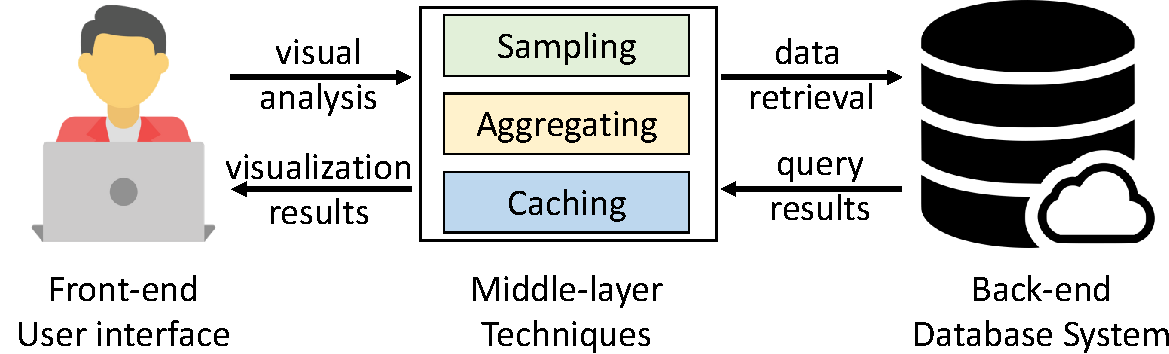
\includegraphics[width=0.40\textwidth]{pictures/framework/framework.pdf}
	\vspace{-2mm}
	\caption{System architecture for interactive visualization.} \label{fig:framework}
    \vspace{-2mm}
\end{figure}


\stitle{Aggregating-based techniques}
%{Aggregating-based techniques pre-process raw data with aggregation techniques (e.g., clustering) in the middle-layer, and yield fewer rendering objects for interactive visual analysis.}
%Returning to the trajectory visual analysis,
These works~\cite{wood2010visualisation,guo2009flow,von2015mobilitygraphs} divide the {spatial space} into basic units and visualize the aggregated information of the trajectories for each unit. For more details on aggregating-based techniques, we refer the reader to the related works~\cite{andrienko2008spatio,adrienko2010spatial}. Our problem and solutions are different from these works as we focus on visualizing the raw input data, instead of the aggregated results.
%However, aggregating-based methods will cause information loss definitely.
%For instance, the continuous spatial traces of the moving objects are always missing and the rarely appeared trajectories are easily to be ignored.






\stitle{Sampling-based techniques}
Sampling techniques are widely used in both visualization and database communities ~\cite{battle2013dynamic,chen2014visual,park2016visualization,qin2020making,DBLP:conf/sigmod/DingHCC016,DBLP:journals/pvldb/KimBPIMR15}.
%are well-studied in the interactive visualization problems with large-scale input data.
%It is
%In particular, ~\cite{chen2014visual} devised a sampling algorithm to preserve the meaningful data items.
% according to the analyzing requirement such as the multi-class data analysis and hierarchical exploration.
The work most relevant to ours is~\cite{park2016visualization}, which is designed for scatter plots (a form of point-based visualization). It solves the problem of point overdrawing and preserves the spatial point distribution of the original dataset at the same time. The techniques in~\cite{park2016visualization} cannot be adapted to our trajectory visualization problem
as trajectory is more complex than scatter points (e.g., varying lengths, contiguous GPS points).
%(i) the complexity of the trajectories~\cite{pelekis2010unsupervised}, and (ii) the loss function and its corresponding solutions are specified for scatter plot, not applicable for line-based trajectory visualization.
%For trajectory visual analysis,  most of the existing trajectory sampling techniques (if not all) cluster the trajectories at first,
%then select the most representative trajectories from each cluster and visualize them.
%It is impractical to provide interactive visualizations for real-world applications as
%trajectory clustering is still an open problem in both database and visualization communities~\cite{panagiotakis2011segmentation,agarwal2018subtrajectory}.

%as
%(i) the trajectory similarity computation and clustering algorithms are very expensive~\cite{pelekis2007similarity},
%and (ii) the



\stitle{Caching-based and other techniques}
%Caching is commonly used to improve the performance of large data processing system, e.g., search engine~\cite{xu2015diversified}.
Chan et al. present ATLAS~\cite{chan2008maintaining}, which utilizes caching for efficient data communication between server and client.
In addition, ATLAS also exploits a powerful multi-core server to accelerate visual analysis task processing from the middle-layer to the back-end.
Piringer et al.~\cite{piringer2009multi} propose a multi-threading architecture for interactive visual exploration,
which utilizes multi-core devices and avoids the pitfalls of multi-threading to provide quick visual feedback.
{Our} techniques in this work are orthogonal to researches in this category.

%Current advancing sampling techniques in the visualization domain are mostly
%Some works design advanced sampling algorithms to preserve the meaningful data items according to the analyzing requirement such as the multi-class data analysis and hierarchical exploration~\cite{chen2014visual}. Furthermore, to the usage of more visual channels of the points other than location such as color~\cite{chen2014visual}, size~\cite{woodruff1998constant} and opacity are discussed.
%Closely related to our work, Park et al.~\cite{park2016visualization} proposed the visualization-aware techniques for the scatter plot.
%
%In comparison with the sampling techniques for scatter plot, the trajectory sampling is more challenging because of the complexity of the trajectories~\cite{pelekis2010unsupervised}.
%
%
%Many exiting visual analytics systems leverage powerful database manage system as the backend to facilitate the fast data processing. Based on the solution proposed in ScalaR~\cite{battle2013dynamic}, a common visualization framework involving sampling technique is illustrated as Figure~\ref{fig:framework}, where a sampling layer is set between the backend and frontend. Since the sampling methods are always designed for complicated task, the algorithms may not be efficient enough to support the interactive data exploration. Thus the cache model is always implemented to save the sampling results. In our scenario, the users query large amount of data(e.g. all Shenzhen trajectories in one week) once and then conduct interactive multi-resolution exploration based on the sampled data, thus the method need to guarantee the visual quality well across different resolutions.
%
%Sampling is a delta-facto solution for the problems with big data. Target at the sampling requirement, the naive solutions such as uniform random sampling cannot generate acceptable because the serious visual information loss. In this section, we first define a loss function to evaluate the visual quality between the visualization results between whole dataset and sampled subset. Then we analyze the hardness of the problem and design algorithms for it.
%
%
%\begin{figure}[t]
%	\centering
%	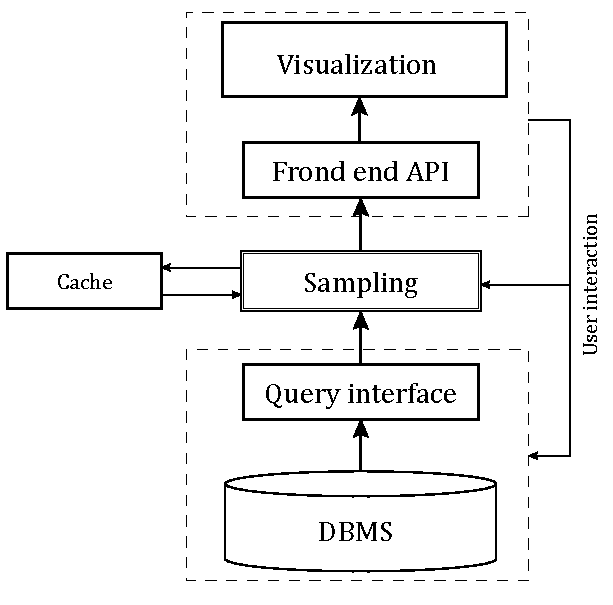
\includegraphics[width=0.3\textwidth]{pictures/framework/DBVAframework.pdf}
%	\vspace{-5mm}
%	\caption{A visualization framework involving sampling layer between the front-end and database management system.}
%	\vspace{-5mm}
%	\label{fig:framework}
%\end{figure}
%

\sstitle{Novelties of our work} To the best of our knowledge, we are the first to observe that random sampling harms visual fidelity for large-scale trajectory visualization and formulate the problem of fidelity-guaranteed sampling. To tackle this problem, we design a complete framework with fidelity loss function, theoretical fidelity loss analysis, and algorithm efficiency optimizations. The well-know visual clutter problem of trajectory visualization is also addressed naturally in our sampling framework. Extensive experimental results show that our proposals effectively maintain visual fidelity and reduces visualization latency at the same time.


%Our work differs from the above researches as we propose visual fidelity-guaranteed sampling approaches for the large-scale trajectory visualization problem,
%we demonstrate the superiority of our proposals by case-, user- and quantitative- studies in real-world dataset.
%
%Unlike existing line-based visualization techniques, we propose visual fidelity-guaranteed sampling approaches for line-based trajectory visualization with large-scale input data.
%To the best of our knowledge, it is the first work which offers theoretical visual fidelity guarantee on the sampling result for large-scale line-based trajectory visualization. 

\section{Problem Formulation}\label{sec:pro}
In this part, we first formally define the \textit{fidelity-optimal sampling problem} in Section~\ref{sec:def} and then show that it is NP-hard to solve the problem exactly in Section~\ref{sec:hard}.

\begin{figure}
	\centering
	\small
	\begin{tabular}{cc}
        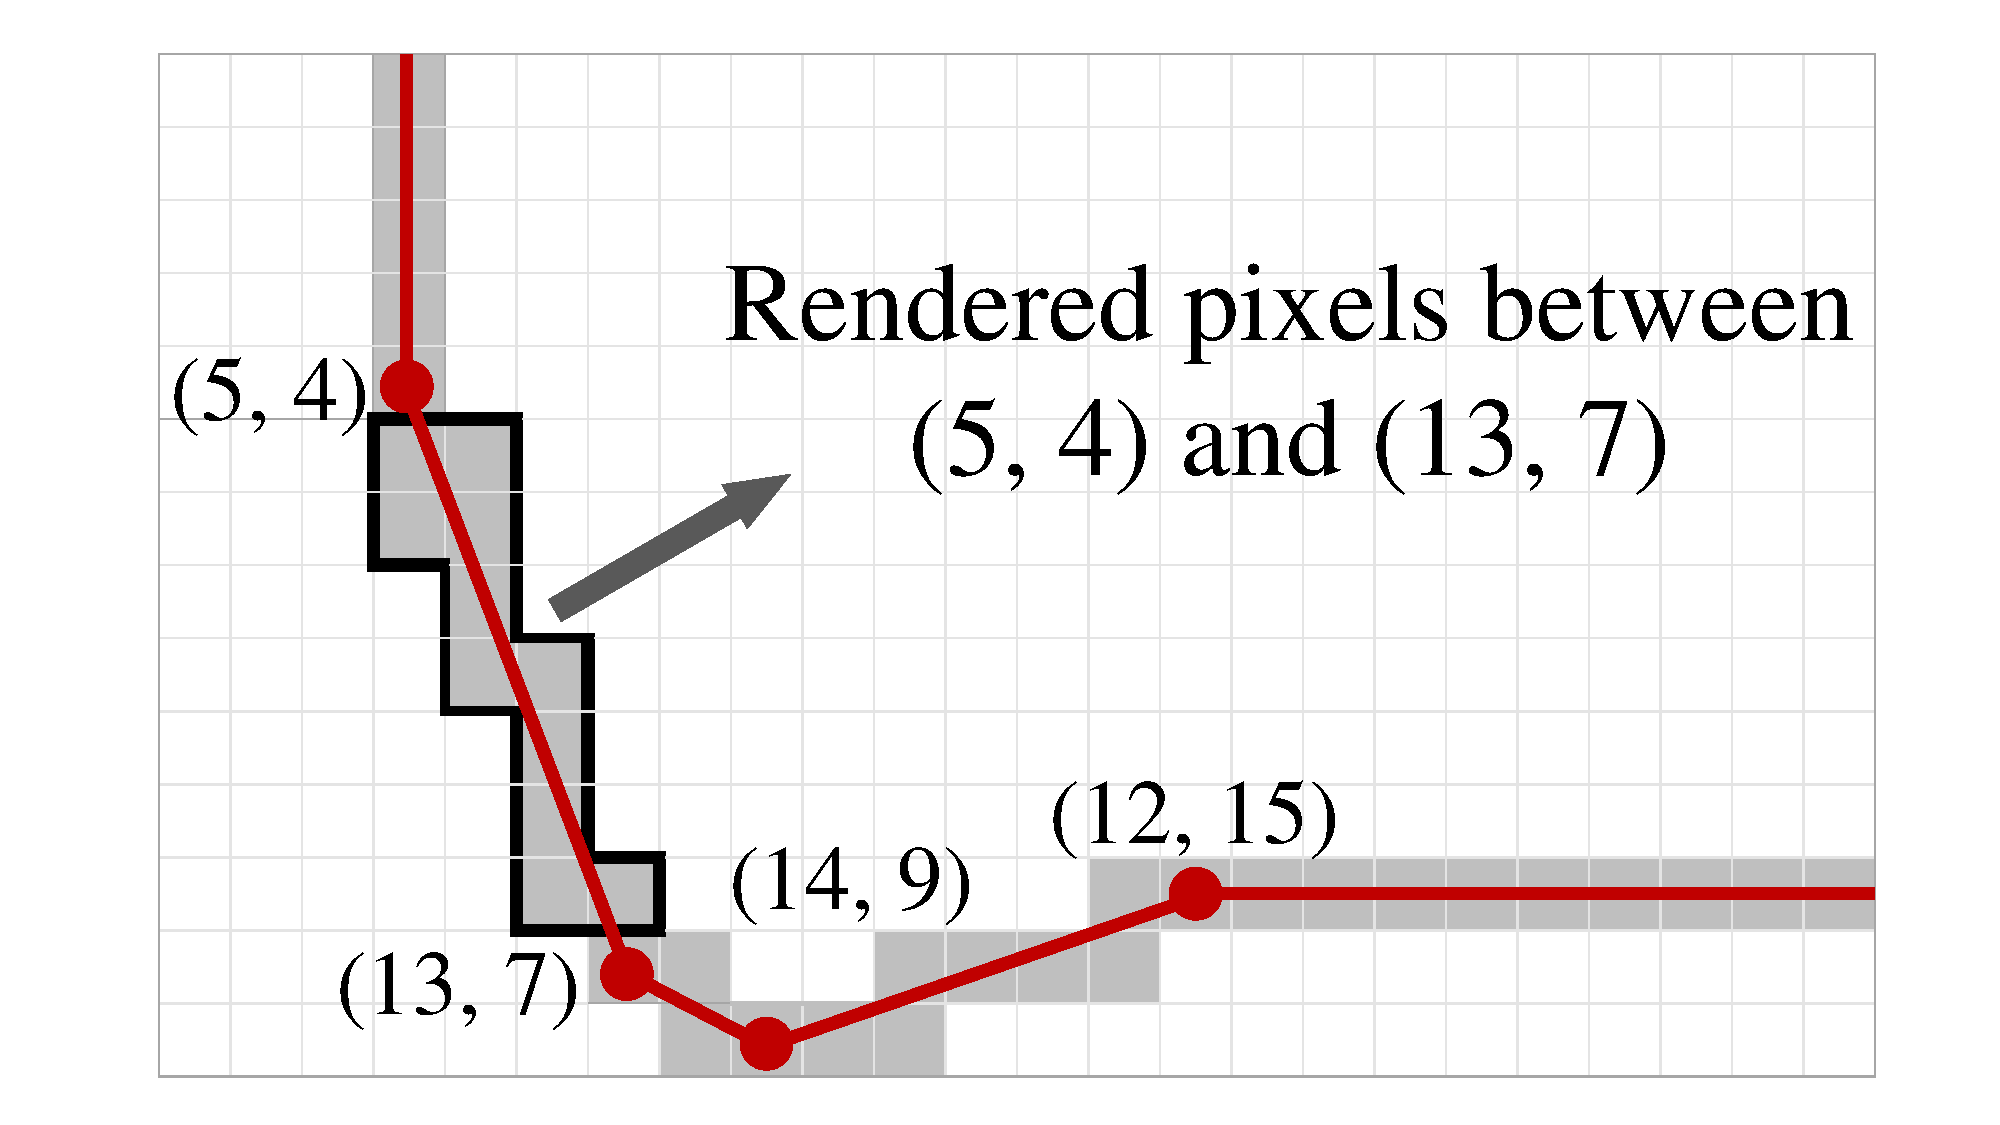
\includegraphics[width=0.43\columnwidth]{pictures/problemsolveing/RenderedPixels}
		&
        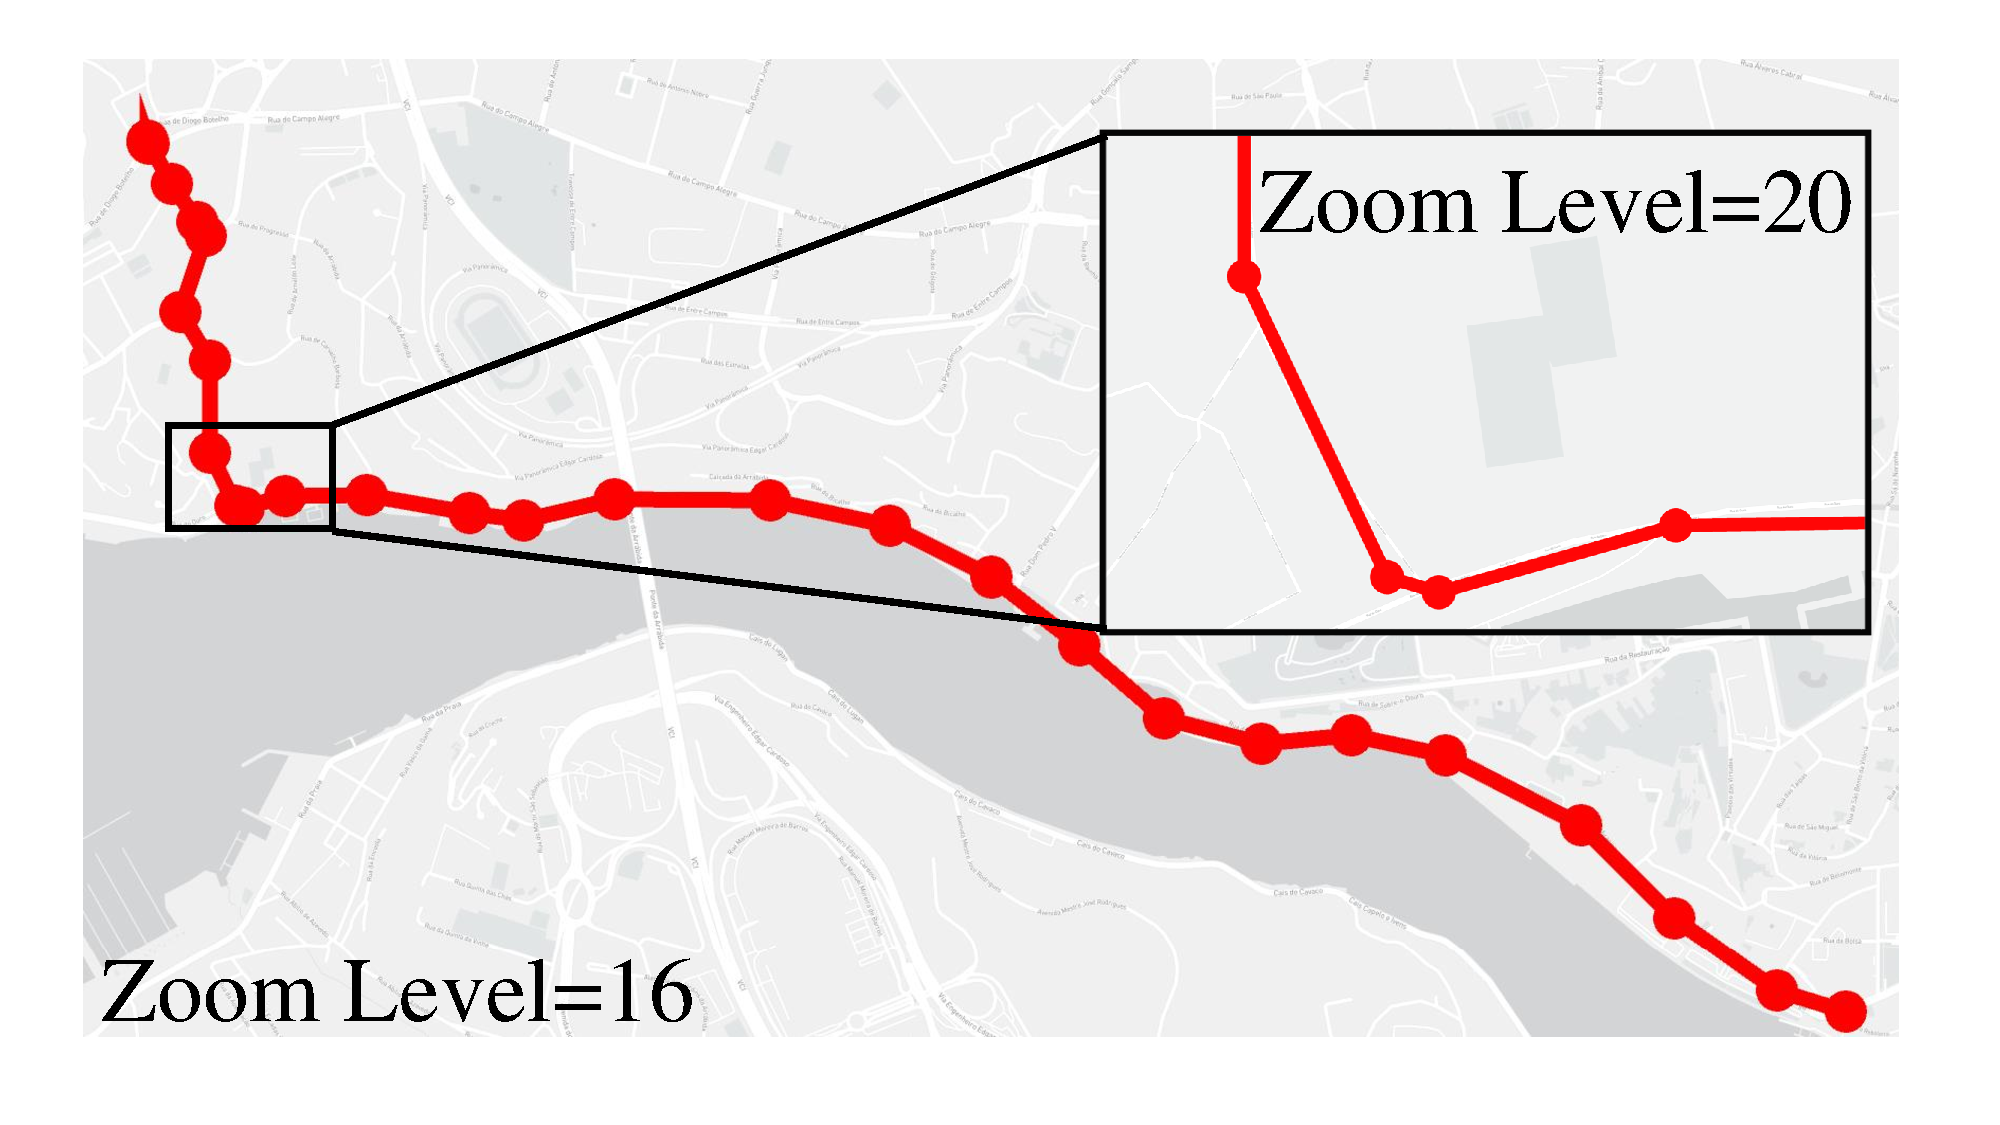
\includegraphics[width=0.48\columnwidth]{pictures/problemsolveing/TrajZoomIn}		
		\\
		(A) Line-based visualization
		&
        (B) Zoom levels
	\end{tabular}
	\vspace{-2mm}
	\caption{Illustration of line-based trajectory visualization.} \label{fig:line}
	\vspace{-2mm}
\end{figure}


\subsection{Problem Definition}\label{sec:def}


We motivate our definition of the \textit{fidelity loss function} by introducing how line-based trajectory visualization works. As introduced earlier, a trajectory contains a sequence of 2-dimensional locations. Given an empty canvas (i.e., the screen of a displaying device) with pixels indexed by horizontal and vertical coordinates (i.e., $x$ and $y$), line-based trajectory visualization connects consecutive locations in each trajectory with polylines and marks the pixels passed by these polylines (with a color different from the background). As shown in Figure~\ref{fig:line}(A), the result of line-based trajectory visualization can be regarded as a 2-dimensional array of boolean variables with 1 indicting a pixel has been marked. Alternatively, we can treat a visualization result $\mathcal{V}$ as a set that contains all marked pixels. This observation leads to the following definition of the fidelity loss function
\begin{equation}\label{eqref:loss}
loss(\mathcal{V}, \mathcal{V}')=\frac{|\mathcal{V}-\mathcal{V}'|}{|\mathcal{V}|},
\end{equation}
in which $|.|$ measures the cardinality of a set, and set $\mathcal{V}^\star=\mathcal{V}-\mathcal{V}'$ contains all distinct elements between $\mathcal{V}$ and $\mathcal{V}'$. We use $loss(\mathcal{V}, \mathcal{V}')$ to measure the fidelity loss of a visualization result $\mathcal{V}'$ compared to the ground-truth visualization $\mathcal{V}$. This definition matches human visual perception as it is essentially the ratio of different pixels in two visualization results. Thus, the approximate visualization $\mathcal{V}'$ will look similar to $\mathcal{V}$ if $loss(\mathcal{V}, \mathcal{V}')$ is small.


Given the fidelity loss function, we are ready to define the fidelity-optimal sampling problem. Denote the set of all trajectories in a dataset as $\mathcal{T}$ and a subset of $\mathcal{T}$ (which contains some sampled trajectories) as $\mathcal{R}$. With a slight abuse of the notation, we use $V(\mathcal{S})$ to denote the visualization results derived from a set $\mathcal{S}$ of trajectories.

\begin{problem}[Fidelity-optimal sampling problem]\label{prob:def}
	Given a sampling rate $\alpha$, find a set $\mathcal{R}$ that satisfies
	\begin{equation}\label{eq:opp}
	\min_{\mathcal{R} \subseteq \mathcal{T}, |\mathcal{R} | = \alpha \mathcal{T} } loss(V(\mathcal{T}), V(\mathcal{R})).
	\end{equation}
\end{problem}
If there is a solution for the above fidelity-optimal sampling problem, to provide a guaranteed fidelity $loss(V(\mathcal{T}), V(\mathcal{R}))\le \tau$, we can simply use a binary search to find the smallest $\alpha$ under which the visual fidelity requirement holds.

One subtlety is that trajectory visualization needs to work at different \textit{zoom levels} upon user request. For example, Google map~\cite{googlemap} provides a zoom levels from 0 to 20, with level 0 providing the largest visualization range (i.e., the whole world) but the lowest resolution, and level 20 providing the smallest visualization range (e.g., individual building, if available) but the highest resolution. We also provided an illustration of zoom level in Figure~\ref{fig:line}(B). Ideally, we want a sample to be \textit{zoom-level-independent}, providing a consistent fidelity guarantee at different zoom levels. This turns out to be straightforward as trajectory visualization merges several pixels in a high-level result (by pixel-wise $OR$) to obtain a pixel in a lower-level visualization result. The following theorem shows that it suffices to satisfy the fidelity guarantee at the highest zoom level.
\begin{theorem}~\label{the:level}
	Use~$loss(V(\mathcal{T}), V(\mathcal{R}), l)$ to denote the fidelity loss induced by a sample set $\mathcal{R}$ at zoom level $l$, we have~ $loss(V(\mathcal{T}), V(\mathcal{R}), l) \\ \le loss(V(\mathcal{T}), V(\mathcal{R}), l')$ if $l\le l'$, with larger $l$ indicating higher resolution.
\end{theorem}

\REPORT{
\begin{proof}
	Denote the value of the pixel at location $(x,y)$ for the visualization result of zoom level $l$ as $p^l(x,y)$, which can be either 0 or 1 in line-based trajectory visualization. Recall that pixels of lower zoom levels are obtained by merging pixels from lower zoom levels with pixel-wise OR. Thus, we have $p^l(x,y)=\vee_{(a,b)\in g(x,y,l,l')} \ p^{l'}(a,b)$, in which  $l\le l'$ and $g(x,y,l,l')$ is the set of pixels in the visualization of zoom level $l'$ that are used to determine $p^l(x,y)$ at zoom level $l$. Use $p^l_{V(\mathcal{S})}(x,y)$ to denote the $p^l(x,y)$ induced by a set $\mathcal{S}$ of sample trajectories, we have 
	$p^l_{V(\mathcal{T})}(x,y)=p^l_{V(\mathcal{R})}(x,y) \ \text{if} \ \exists (a,b)\in g(x,y) \ \text{~~such that~~} p^{l'}_{V(\mathcal{T})}(x,y)=p^{l'}_{V(\mathcal{R})}(x,y).$ It follows that 
	
	$loss(V(\mathcal{T}), V(\mathcal{R}),l)=\frac{|V^l(\mathcal{T})-V^l(\mathcal{T})|}{|V^l(\mathcal{T})|}\le \frac{|V^{l'}(\mathcal{T})-V^{l'}(\mathcal{T})|}{|V^{l'}(\mathcal{T})|}=\\loss(V(\mathcal{T}), V(\mathcal{R}), l').$

\end{proof}
}

We are aware that lower zoom levels need more coarse-grained visualization and thus the sampling rate at the highest level may be larger than necessary. We left more sophisticated designs, such as re-sampling a sample set or generating multiple sample sets for future work, and consider only sampling for the highest zoom level. As our fidelity loss function considers the entire visible region (i.e., it is a \textit{global fidelity measure}), the visual difference between our sample and the ground-truth visualization may be large for some specific regions, especially when the marked points are sparse in these regions. \textit{Local visual fidelity} can be important for some tasks(e.g., outlier discovery~\cite{feng2010matching,mayorga2013splatterplots}) and we leave it for future work. We want to note that a fidelity-guaranteed sample $\mathcal{R}$ is also \textit{query independent} from the definition of the fidelity loss function, which means $\mathcal{R}$ only needs to be constructed once to answer all queries.






\subsection{Hardness Analysis}\label{sec:hard}
We use $t_i \in \mathcal{T}$ to denote a trajectory in the dataset. According to the working mechanism of line-based trajectory visualization, $t_i$ corresponds to a set of marked pixels on the canvas in the ground-truth visualization and we also use $t_i$ to denote this set of pixels. Thus, we have $V(\mathcal{T}) = \cup_{t_i \in \mathcal{T}} t_i$ and $V(\mathcal{R}) = \cup_{t_i \in \mathcal{R}} t_i$. We can transform Problem~\ref{prob:def} as follows

\begin{align}\label{eqn:obj2} \nonumber
\min_{\oR \subseteq \D, |\oR| = \alpha |\D|}  \frac{|\V(\D) - \V(\oR)|}{|\V(\D)|}  & \Leftrightarrow \min_{\oR \subseteq \D, |\oR| = \alpha |\D|}   - |\V(\oR)| \\ \nonumber
 \Leftrightarrow \max_{\oR \subseteq \D, |\oR| = \alpha |\D|}  |\V(\oR)| &  \Leftrightarrow \max_{\oR \subseteq \D, |\oR| = \alpha |\D|} | \cup_{t_i \in \oR} t_i |
\end{align}

The above transformations use the fact that $V(\mathcal{R}) \subset V(\mathcal{T})$ as $\mathcal{R} \subset \mathcal{T}$, and the ground-truth set $V(\mathcal{T})$ is constant. The last line shows that fidelity-optimal sampling is equivalent to the well-known set cover maximization problem.
Specifically, given an integer $k = \alpha |\D|$, and a collection trajectory pixel set $\D = \{t_1, t_2, \cdots, t_n \}$, set cover maximization finds a subset $\oR \subset \D$ such that $|\oR| \leq k$ and $|\cup_{t_i \in \oR} t_i|$ is maximized. The set cover maximization problem is well-known to be NP-hard~\cite{setcover}.


%It is equivalent to select sized-$k$ trajectory set $\oR$ from $\D$ which $\cup_{\oR_i \in \oR} \oR_i$ is maximized.
%It is a NP-hard problem as we proved in Lemma~\ref{lem:np}.

%\begin{lemma}[NP hard]~\label{lem:np}
%Given a trajectory dataset $\D$ and an integer $k$,
%The sampling-based trajectory visualization problem (see Problem~\ref{prob:def}) is NP-hard.
%\end{lemma}

%We omit the proof of Lemma~\ref{lem:np} as it is a typical set cover maximization problem\footnote{\url{https://en.wikipedia.org/wiki/Maximum_coverage_problem}}, which is a well-known NP-hard problem in literature.

%------------comments by Bo-------------------
%As we analyzed in Section~\ref{sec:intro}, the large-scale (e.g., hundreds of millions GPS points) line-based trajectory visualization problem is very challenging due to the large data size and limited rendering capability of graphics devices.
%To make matters worse, the visualization result of large-scale trajectory dataset suffers visual clutter seriously.
%In this work, we focus on how to visualize large-scale trajectory dataset efficiently and effectively.
%In particular, our objective is to devise a visual fidelity guaranteed sampling method for large trajectory data visualization.
%The major challenges to achieve this goal are:
%(i) how to define visual fidelity theoretically? (ii) how to guarantee the visual fidelity of the sampling-based visualization result?


%\section{Visual Fidelity Guaranteed Sampling Approach}\label{sec:sol}
\section{Our Solution: $\vats$}\label{sec:sol}
In this section, we focus on addressing the second technical challenge: \emph{how to devise an efficient sampling algorithm that provides guaranteed visual fidelity?}
Specifically, we first propose a visual fidelity-guaranteed sampling algorithm $\vats$ in Section~\ref{sec:greedy}. Next, we devise several optimizations to improve the efficiency of $\vats$ in Section~\ref{sec:opt}.

\subsection{Visual Fidelity-Guaranteed Sampling}\label{sec:greedy}
Due to the hardness of Problem~\ref{prob:def}, the straight-forward solution is uniform random sampling $\rand$.
This solution randomly selects $k$ trajectories from the dataset $\D$ and stores them in the result set $\oR$. The selected trajectories in $\oR$ are rendered as the visualization result.
Obviously, uniform random sampling $\rand$ does not provide any guarantee on the visual fidelity of the sampled set.

We next present our visual fidelity-guaranteed sampling method $\vats$ in Algorithm~\ref{alg:greedy}, which employs a greedy paradigm.
In particular, it finds the trajectory $tmp$ in $\D$ that maximizes $|\oR \cup tmp|$ at each iteration, as shown in Line~\ref{line:max} of Algorithm~\ref{alg:greedy}.
It terminates after $k=\alpha |\D|$ iterations and returns $\oR$ as the result set for rendering.

%\vspace{-2mm}
\begin{algorithm}
    \caption{$\vats(\D,k=\alpha |\D|)$} \label{alg:greedy}
    \begin{algorithmic}[1]
    \State Initialize result set $\oR \leftarrow \emptyset$
    \While{$|\oR| < k$}
        \State $tmp \leftarrow argmax_{t_i \in \D} |\oR \cup t_i|$ \label{line:max}
        \State $\oR \leftarrow \oR \cup \{ tmp \}$
    \EndWhile
    \State Return $\oR$
    \end{algorithmic}
\end{algorithm}


Interestingly, Algorithm~\ref{alg:greedy} provides provable visual fidelity guarantee for the returned result $\oR$, as stated in Theorem~\ref{the:ratio}.
%~\footnote{We omitted all the proofs of the theorems and lemmata in this work due to space reasons, and refer the interested readers to our technical report\cite{techreport}.}

\begin{theorem}~\label{the:ratio}
Define the visual fidelity of a sample set $\mathcal{S}$ as $f(\mathcal{S})=1-loss(\V(\D),\V(\mathcal{S}))$. Let the sized-k result produced by Algorithm~\ref{alg:greedy} be $\mathcal{R}$ and the sized-k solution of Equation~\eqref{eq:opp} be $\mathcal{R}^{\star}$, we have $f(\mathcal{R})\ge 0.632*f(\mathcal{R}^{\star})$.
\end{theorem}

\REPORT{
\begin{proof}
The optimal solution of Problem~\ref{prob:def} covers $OPT$ pixels in $k$ iterations.
Let $a_i$ be the number of newly covered pixels at the $i$-th iteration, $b_i$ is the total number of covered pixels up to the $i$-th iteration (i.e., $b_i = \sum_{j=1}^{i}a_i$),
and $c_i$ be the uncovered pixels after $i$-th iteration (i.e., $c_i = OPT-b_i$).
According to greedy paradigm, we can conclude the number of newly covered pixels at the $(i+1)$-th iteration is always greater than or equal to $\frac{1}{k}$ of the number of uncovered pixels after the $i$-th iteration, i.e., $a_{i+1} \geq \frac{c_i}{k}$.
We prove Theorem~\ref{the:ratio} by proving $c_{i+1} \leq (1-1/k)^{i+1} \cdot OPT$.
It holds $c_1 \leq (1-1/k) \cdot OPT$ as follows.
\begin{align} \nonumber
& a_1 \geq c_0 \cdot 1/k = 1/k \cdot OPT \text{~~~as we concluded~~~} a_{i+1} \geq \frac{c_i}{k}\\ \nonumber
 \Leftrightarrow  & b_1 \geq 1/k \cdot OPT  \Leftrightarrow  -b_1 \leq - 1/k \cdot OPT  \text{~~~as~~~} a_1 = b_1\\ \nonumber
 \Leftrightarrow & OPT - b_ 1 \leq OPT - 1/k \cdot OPT  \Leftrightarrow  c_1 \leq (1-1/k) \cdot OPT
\end{align}
For inductive hypothesis assume $c_{i} \leq (1-1/k)^i \cdot OPT$. Thus,
\begin{align} \nonumber
& c_{i+1} = c_i - a_{i+1} \leq c_i - c_i/k = (1-1/k) \cdot c_i = (1-1/k)^{i+1} \cdot OPT
\end{align}

Hence, it holds $c_k \leq (1-1/k)^{k} \cdot OPT$.
It is equivalent to $b_k \geq (1 - (1-1/k)^{k}) \cdot OPT \geq (1-1/e) \cdot OPT \approx 0.632 \cdot OPT$.
\end{proof}
}

\subsection{Optimization Techniques}\label{sec:opt}
With the above theoretical analysis, Algorithm~\ref{alg:greedy} offers a visual fidelity-guaranteed sampling algorithm for the large-scale trajectory data visualization problem.
However, as the time complexity analyzed in Lemma~\ref{lem:cost}, it is not scalable to large-scale trajectory datasets (e.g., millions of trajectories).

% as the time complexity analyzed in the following Lemma~\ref{lem:cost}.
\begin{lemma}[Time Complexity]~\label{lem:cost}
Given trajectory dataset $\D$ and an integer $k = \alpha |\D|$, the time complexity of Algorithm~\ref{alg:greedy} is $O(\alpha \cdot m \cdot |\D|^2)$, where $m$ is the maximum length of all trajectories in dataset $\D$.
\end{lemma}

\REPORT{
\begin{proof}
At each iteration ($k = \alpha |\D|$ iterations in total),
it computes the uncovered pixels of each trajectory in dataset $\D$ with $O(m)$ cost.
The dataset $\D$ has $O(|\D|)$ trajectories.
Thus, the total cost is $O(k \cdot m \cdot |\D|)=O(\alpha \cdot m \cdot |\D|^2)$.
\end{proof}
}

For example, the \pt{} trajectory dataset has 2.39 millions of taxi trajectories.
The maximum length of the trajectories in it has 3,490 GPS points.
It takes 413.6 seconds to return a subset $\oR$ with sampling rate $0.1\%$.
Obviously, it is impractical for interactive trajectory explorations.

Due to the inefficient of our visual fidelity-guaranteed sampling approach in Algorithm~\ref{alg:greedy},
we then devise performance optimization techniques to accelerate its running time.
The core idea is utilizing the submodularity of the covered pixels of result set $\oR$, as shown in Lemma~\ref{lem:submodular}.


\begin{lemma}[Submodularity]\label{lem:submodular}
Define the contribution of a trajectory $t$ to the result set $\oR$ as $\Delta(\oR, t) = |V(\oR \cup t)| - |V(\oR)|$.
Given a trajectory $t$ and two result sets $\oR,\oR^{'}$, if $\oR \subset \oR^{'}$, then $ \Delta(\oR, t) \geq \Delta(\oR^{'}, t)$.
\end{lemma}


\REPORT{
\begin{proof}
The contribution value of trajectory $t$ to a given result set $\oR$ (e.g., $\Delta(\oR, t) = |\oR \cup t| - |\oR|$) is the new covered pixels of $t$ w.r.t. result set $\oR$, i.e., $|t| - |\oR \cap t|$.
It holds $t \cap \oR \subseteq  t \cap \oR^{'}$ as $\oR^{'}$ is a superset of $\oR$.
Thus, we have $|t| - |t \cap \oR| \geq |t| - |t \cap \oR^{'}|$.
Hence, it holds $\Delta(\oR, t) = |\oR \cup t| - |\oR| \geq |\oR^{'} \cup t| - |\oR^{'}|= \Delta(\oR^{'}, t)$.
\end{proof}
}

\begin{figure}
 \centering
 \small
 \begin{tabular}{cc}
   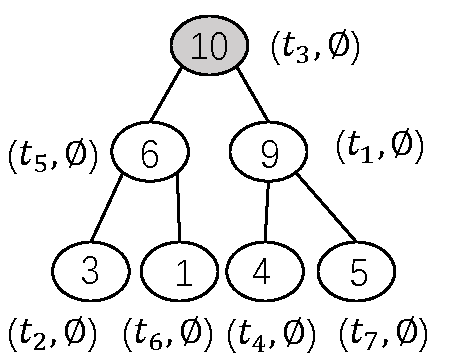
\includegraphics[width=0.35\columnwidth]{pictures/1st}
   &
   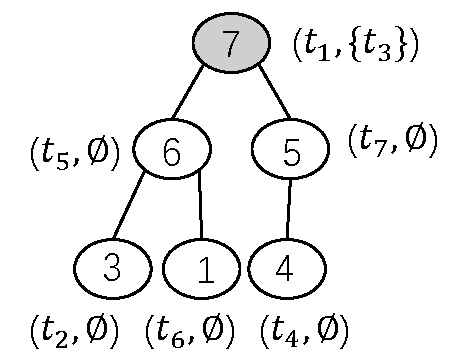
\includegraphics[width=0.35\columnwidth]{pictures/2nd}
   \\
   (A) 1st iteration
   &
   (B) 2nd iteration
 \end{tabular}
 \vspace{-3mm}
 \caption{Lazy computing manner.} \label{fig:heap} %via the submodularity in Lemma~\ref{lem:submodular}
 \vspace{-6mm}
\end{figure}


The submodularity in Lemma~\ref{lem:submodular} reduces many unnecessary trajectory contribution value computations.
We maintain a max-heap for the number of uncovered pixels of each trajectory and employ a lazy computing manner.
That is, the contribution of a given trajectory is computed when necessary.
Figure~\ref{fig:heap}(a) shows a tiny max-heap example about the numbers of uncovered pixels of each trajectory from $t_1$ to $t_7$ with result set $\oR=\emptyset$.
At the first iteration, the root node of the max-heap, $t_3$ in Figure~\ref{fig:heap}(A), is selected.
At the second iteration, the number of uncovered pixels of the root node $t_1$ is updated to 7 w.r.t. result set $\oR = \{t_3 \}$ (see gray node at Figure~\ref{fig:heap}(B)).
Then $t_1$ is selected at the second iteration without computing the number of uncovered pixels in other trajectories, i.e., all white nodes at Figure~\ref{fig:heap}(B).
The reason is that the contribution of the trajectories in all white nodes is less than 7 according to the submodularity in Lemma~\ref{lem:submodular}.

%In summary, the number of uncovered pixels in each trajectory will only be computed with the latest result set $\oR$ when it is necessary in the lazy computing manner,
%e.g., only $t_1$ will be updated at the 2nd iteration in Figure~\ref{fig:heap}.
%It reduces many unnecessary computations through the lazy updating manner, e.g., all white nodes did not update at the 2nd iteration in the above example.

%We then analyze the time complexity of Algorithm~\ref{alg:greedy} with lazy computing manner in Theorem~\ref{lem:lazy}.
%
%\begin{lemma}[Optimized Time Complexity]~\label{lem:lazy}
%Given trajectory dataset $\D$ and an integer $k= \alpha |\D|$, the time complexity of Algorithm~\ref{alg:greedy} with lazy computing manner is $O(\alpha \cdot m \cdot x |\D| \log |\D|)$, where $x$ is the number of contribution computations among all $k$ iterations and $x \ll |\D|$.
%\end{lemma}
%
%\begin{proof}
%It first takes $O(|\D|)$ time to construct the max-heap~\cite{cormen2009introduction}.
%It incurs $O( m \cdot x \log |\D|)$ cost to select the trajectory with maximum uncovered pixels at each iteration ($k$ iterations in total).
%Hence, the overall cost is $O(|\D| + k \cdot m \cdot t \log |\D|)$.
%\end{proof}
The performance of Algorithm~\ref{alg:greedy} is improved significantly because its contribution values are computed only when necessary.
To exemplify, Algorithm~\ref{alg:greedy} costs 413.6 seconds to return the results with sampling rate $0.1\%$ on the \pt{} taxi trajectory dataset.
However, it only needs 1.2 seconds in our performance-optimized $\vats$.


\section{Advanced Approach: $\avats$}\label{sec:aa}
Until now, $\vats$ in Algorithm~\ref{alg:greedy} offers a visual fidelity-guaranteed sampling approach for the large-scale trajectory visualization problem (Problem~\ref{prob:def}),
which returns the fidelity-guaranteed result efficiently via the optimization techniques in Section~\ref{sec:opt}.
%It means that the challenges (i) large trajectory dataset and (ii) limited rendering capability of graphics device (see Section~\ref{sec:intro}) have been addressed.
In this section, we focus on the third technical challenge: \emph{how to tackle the visual clutter problem in large trajectory visualization}?
In particular, we devise the advanced approach $\avats$ to alleviate it by considering
(i) trajectory data distribution, and (ii) human perception capability.
We elaborate (i) and (ii) by the examples in Figure~\ref{fig:delta} shortly.


\stitle{Trajectory data distribution} Considering the \pt{} trajectory dataset, Figure~\ref{fig:delta}(A) is the visualization result of $\vats$ with sampling ratio $0.5\%$.
Obviously, the real-world trajectory dataset is non-uniform distributed.
For example, the trajectories in dense region are much more than those in the sparse region, as illustrated by the rectangles in Figure~\ref{fig:delta}(A).

\stitle{Human perception capability} Intuitively, humans can more easily distinguish the difference between sparse regions rather than dense regions in Figures~\ref{fig:delta}(A) and (B).
The core reason is the limited perception capability of human beings.
In particular, the visual difference of human beings diminishes when the visualized trajectories are large enough with a given zoom level.
For example, the difference between two dense regions in Figures~\ref{fig:delta}(A) and (B) almost cannot be recognized by human beings.


\begin{figure}%[t]
	\centering
	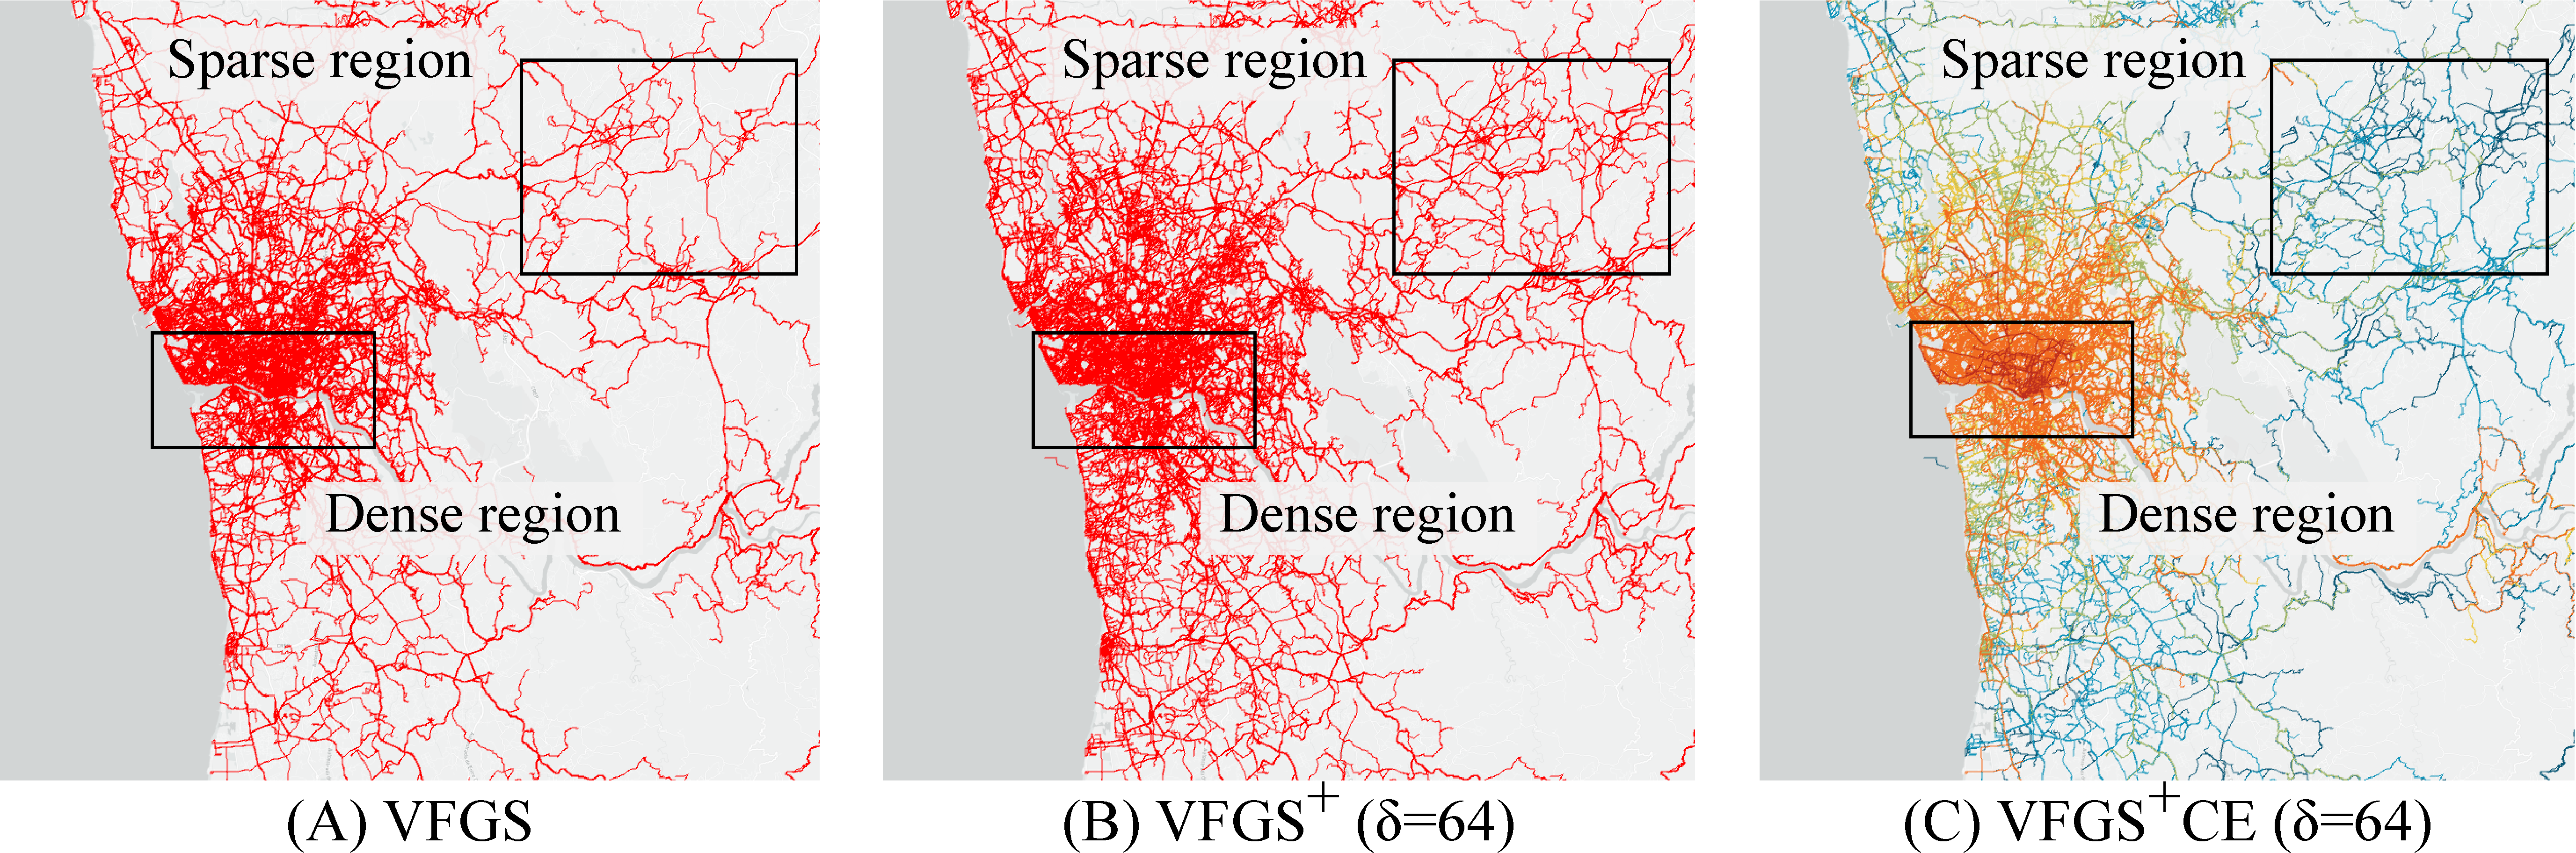
\includegraphics[width=0.48\textwidth]{pictures/problemsolveing/delta_motivation.pdf}
    \vspace{-4mm}
	\caption{The advanced approach $\avats$ on \pt{} ($\alpha = 0.5\%$).} \label{fig:delta}
	 \vspace{-4mm}
\end{figure}

%(see Algorithm~\ref{alg:plus})

Taking the above two observations into consideration, we can further improve the returning result of visual fidelity-guaranteed sampling approach $\vats$ by
delivering rich information at sparse regions and reducing visual clutter in dense regions.
In this section, we devise the advanced approach $\avats$ (see Algorithm~\ref{alg:plus})  to achieve the above two objectives.
In specific, we introduce perception tolerance parameter $\delta$ in $\avats$, which models the perception capability of humans at the highest level of details.
In other words, suppose the pixel $(x,y)$ in canvas is covered by the result set $\oR$ at the highest level,
the pixels around $(x,y)$, i.e., from $(x-\delta, y-\delta)$ to $(x+\delta, y+\delta)$, are not necessary to cover because they are in the perception tolerance of human beings.

Fortunately, we can slightly revise $\vats$ in Algorithm~\ref{alg:greedy} to incorporate the perception tolerance parameter $\delta$ in advance approach $\avats$, as shown in Algorithm~\ref{alg:plus}.
It measures the contribution of each trajectory $t_i$ w.r.t the augmented set $\oR^{+}$ in Line~\ref{line:deltamax},
where $\oR^{+}$ includes both the selected trajectories and their tolerance pixels (in Line~\ref{line:delta}).
%It measures the contribution of each trajectory $t_i$ w.r.t the selected trajectory set $\oR$'s augmented set $\oR^{+}$, i.e., the selected trajectories and their tolerance pixels.
%.
%The augmented set $\oR^{+}$ will be updated by the selected trajectory $tmp$ and its tolerance pixels set (in Line~\ref{line:delta}).

%
\begin{algorithm}
    \caption{$\avats(\D,k=\alpha |\D|,\delta)$} \label{alg:plus}
    \begin{algorithmic}[1]
    \State Initialize result set $\oR \leftarrow \emptyset$
    \State Initialize augmented result set $\oR^{+} \leftarrow \emptyset$
    \While{$|\oR| < k$}
        \State $tmp \leftarrow argmax_{t_i \in \D} \oR^{+} \cup t_i$ \label{line:deltamax}
        \State $\oR \leftarrow \oR \cup \{ tmp \}$
        \State $\oR^{+} \leftarrow \oR^{+} \cup \mathsf{augment}(tmp, \delta)$\label{line:delta}
    \EndWhile
    \For{each $t$ in $\D$} \Comment{Representative encoding} \label{line:s}
        \State $tr \leftarrow argmin_{t_i \in \oR}{\mathsf{augment}(t_i, \delta) - t}$
        \State $tr.\mathsf{cnt}++$ \label{line:e}
    \EndFor
    \State Return $\oR$
    \end{algorithmic}
\end{algorithm}


Interestingly, the visual clutter large trajectory visualization problem can be further reduced
by encoding representative trajectories in $\oR$ (the returning result of $\avats$) with colors.
In particular, $\avats$ selects the trajectory with the largest uncovered pixels by taking the perception tolerance capability of humans into account at each iteration,
instead of only choosing the trajectory with the largest uncovered pixels in $\vats$ (Algorithm~\ref{alg:greedy}).
During its selection process, some trajectories will not be included into the result set $\oR$ even they have more uncovered pixels w.r.t. $\oR$.
The reason is their uncovered pixels are too close to the pixels in the selected trajectories (i.e., within the tolerance area of selected pixels).
With Figure~\ref{fig:zoom}(A) as an example, suppose $\delta=1$ and trajectory $a$ was selected at the first iteration,
the selected trajectory in the second iteration is $c$ instead of $b$ because almost all pixels in $b$ is in the tolerance area of $a$'s.

Inherently, the $\avats$ trajectory selection process embeds the representativeness of each trajectory in the result set $\oR$.
We define the representativeness of a trajectory as the number of influenced trajectories in the dataset $\D$.
We compute the representativeness of each trajectory in $\oR$ from Line~\ref{line:s} to Line~\ref{line:e} in Algorithm~\ref{alg:plus}, then visualize them by encoding with different colors.
Figure~\ref{fig:delta}(C) shows the visualized result of $\avats$ by encoding the trajectory representativeness with colors.
Obviously, the trajectories in dense region are darker than those in sparse region, indicating there are more trajectories in dense region.
%Thus, the selected trajectories in the dense region are more representative than those in sparse region.

\begin{figure}[t]
	\centering
	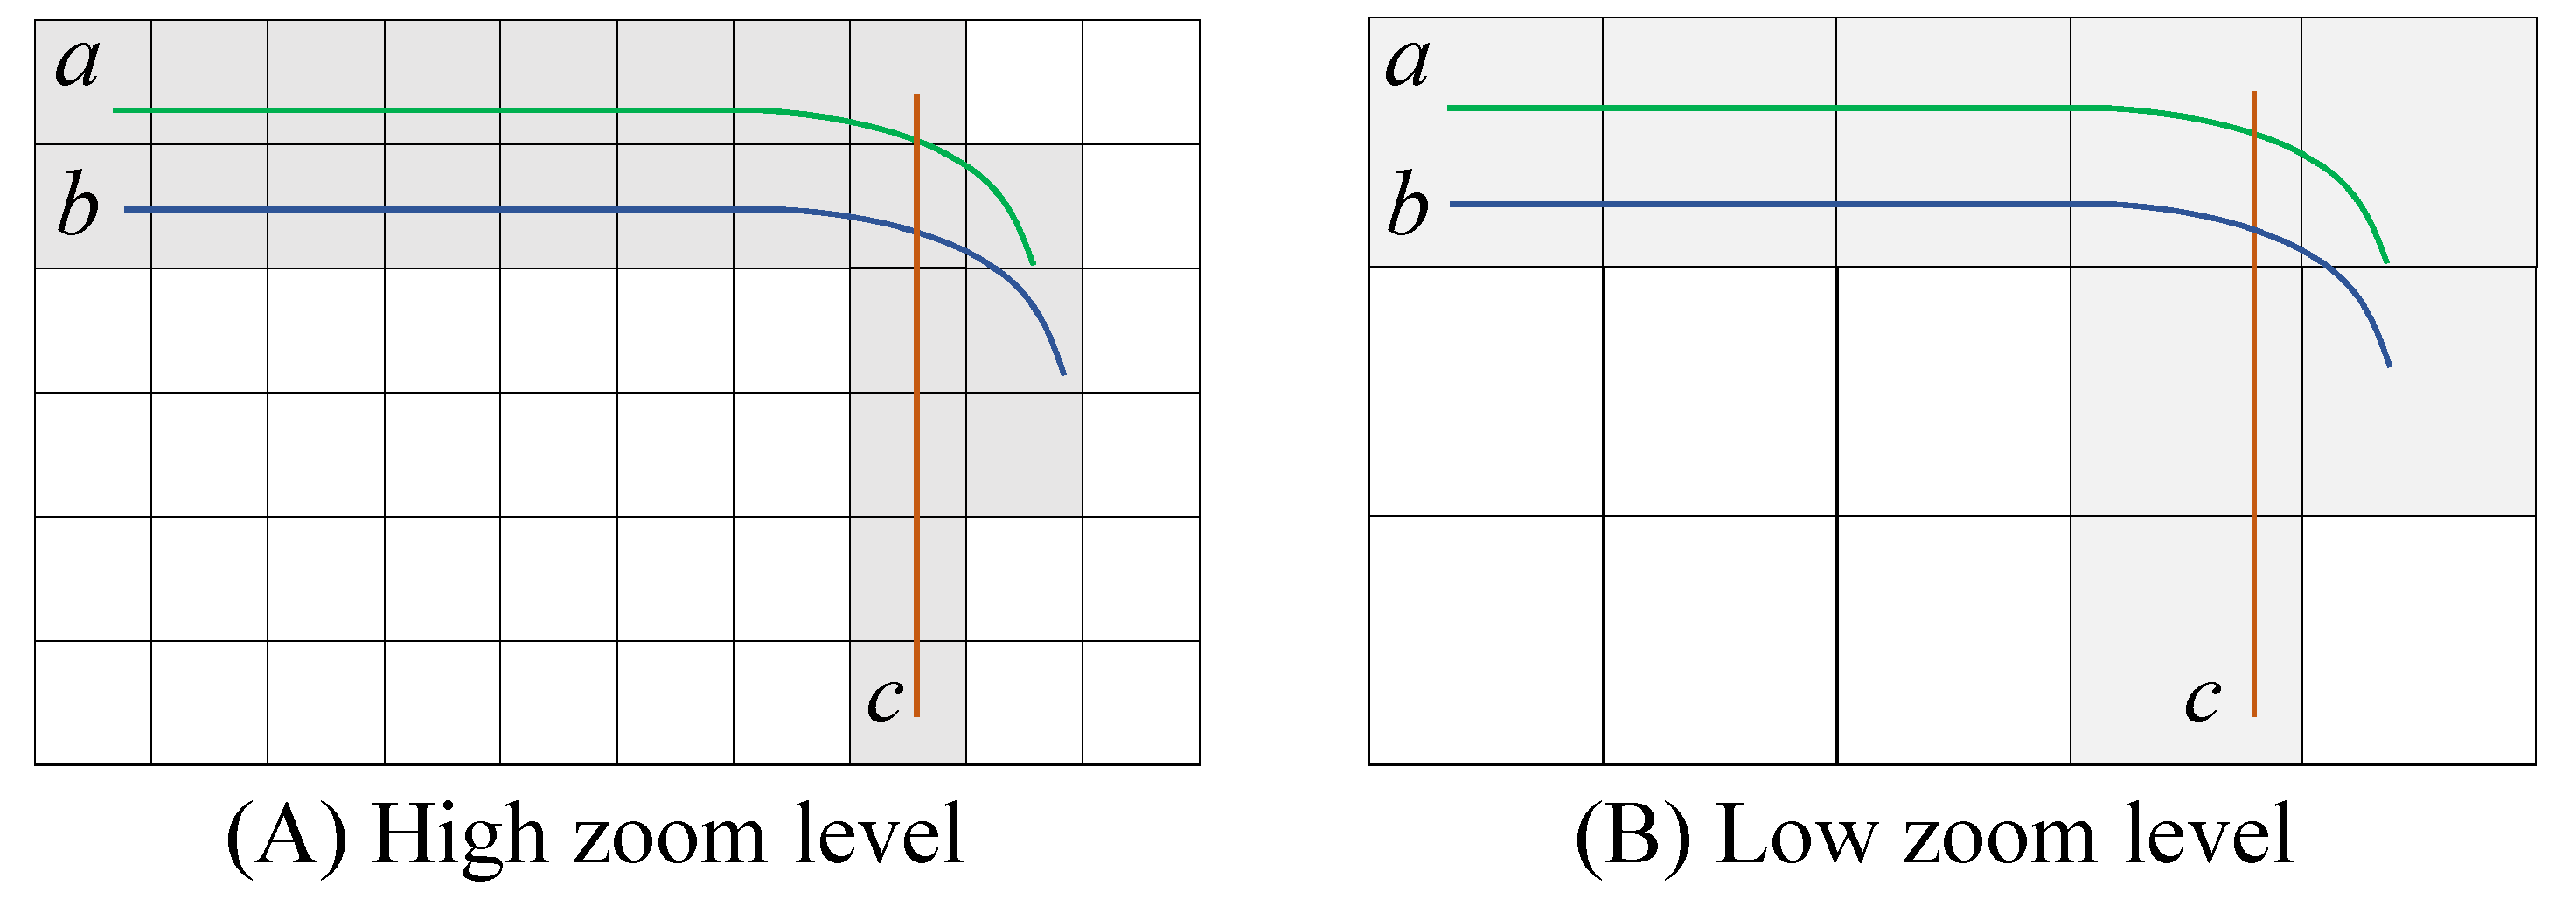
\includegraphics[width=0.45\textwidth]{pictures/problemsolveing/one_to_many.pdf}
	\vspace{-2mm}
	\caption{$\avats$ at different zoom levels.}	\label{fig:zoom} %An illustration of
    \vspace{-2mm}
\end{figure}


Notably, $\avats$ provides excellent visual fidelity over $\vats$ at arbitrary zooming resolutions naturally.
The key technique to achieve that is it considers the zooming resolutions inherently when introducing the perception tolerance $\delta$.
For example, the zoom level in Figure~\ref{fig:zoom}(A) is higher than that in Figure~\ref{fig:zoom}(B).
As our above elaboration, $\avats$ selects trajectory $a$ and $c$ at Figure~\ref{fig:zoom}(A).
When it zoomed out, as shown in Figure~\ref{fig:zoom}(b), it still captures the main sketch of the underlying dataset (as gray cells shown).
We will elaborate it by the experimental study in Section~\ref{sec:exp}.




%(1) Richer Information Delivering: details aware; so Arbitrary zooming resolutions
%(2) Popularity Embedding: visual clutter



%\subsection{One-to-many strategy}~\label{sec:one_to_many}
%Since we detect the covered pixels in the highest level, two trajectories may be very close to each other but share very few pixels, which will lead to more information loss in the low zoom view as figure~\ref{fig:one_to_many}.
%We next elaborate a ``one-to-many'' strategy to further optimize the visual quality of our proposed technique.
%Recalling we use the highest zoom level to define the pixel size in the canvas.
%Thus, our visual quality guaranteed sampling algorithm is zoom-level oblivious, e.g., it guarantees the visual quality of result set $\oR$ at every zoom level.
%However, users always do not use/need the highest zoom level in visualization applications.
%For example, Google map shows city and streets at zoom level 1 and 15, respectively~\footnote{\url{https://developers.google.com/maps/documentation/}}.
%Motivated by the above observation, we devise ``one-to-many'' strategy by introducing a visual tolerance parameter $\delta$ to optimize the visual quality for users.
%Specifically, ,
%the ``one-to-many'' strategy will ignore all the pixels around $(x,y)$ within $\delta$ offset distance, i.e., all pixels from $(x-\delta, y-\delta)$ to $(x+\delta, y+\delta)$ will be skipped.
%We will demonstrate the effectiveness of the visual tolerance $\delta$ in experimental evaluations.
%
%%https://developers.google.com/maps/documentation/maps-static/dev-guide#Zoomlevels
%\begin{figure}[t]
%	\centering
%	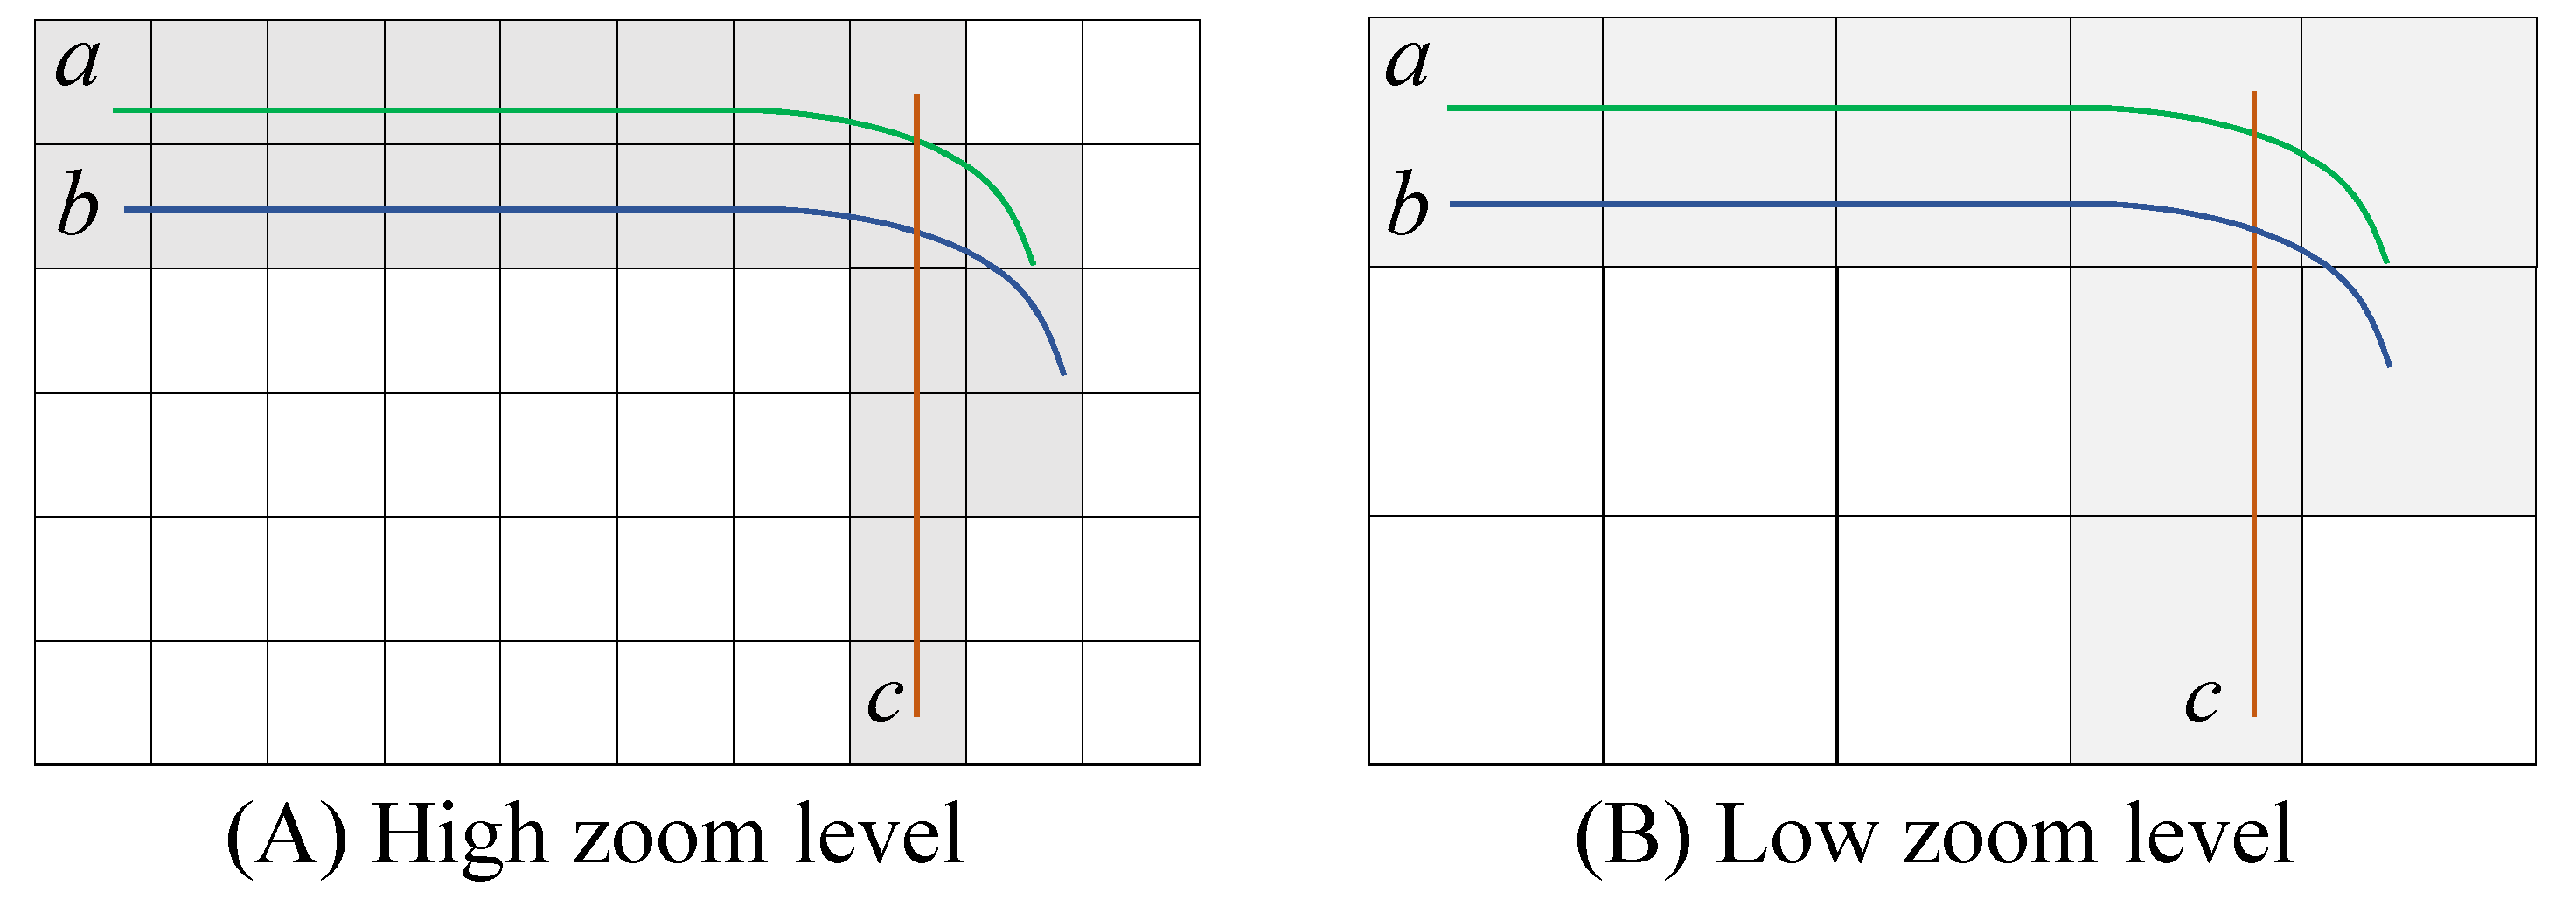
\includegraphics[width=0.4\textwidth]{pictures/problemsolveing/one_to_many.pdf}
%	\vspace{-5mm}
%	\caption{Resolution inconsistency}
%	\vspace{-5mm}
%	\label{fig:one_to_many}
%\end{figure}


%Specifically, $\avats$ incorporates a parameter $\delta$ during trajectory selection process in $\vats$ .
%In particular, we employ the parameter $\delta$ to model the end user's perception ability at the most high level of details.
%Surprisingly, our advance approach $\avats$ not only provides better visualization result when comparing with $\vats$ with the same sampling rate
%(e.g., Figure~\ref{fig:delta}(a) and (b) are the returning result of $\vats$ and $\avats$ respectively),
%but also embeds the popularity of selected trajectories by encoding the rest trajectories in the dataset in them,
%e.g., Figure~\ref{fig:delta}(c) is the visual result of $\avats$ with color encoded popularity.





\section{Experimental Evaluation}\label{sec:exp}


We evaluate our techniques on two real-world trajectory datasets: \pt{} and \sz{}.
\pt{}~\cite{pt} contains a total of 2.39 million taxi trajectories and 75.67 million of GPS points, and the longest trajectory has 3,490 GPS points.
\sz{}~\cite{sz} consists of 3.07 million taxi trajectories with 53.53 million GPS points, and the longest trajectory has 2,268 GPS points. All experiments are conducted on a machine with an Intel i7-8700 CPU, 24 GB memory and an NVIDIA GeForce GTX1080 GPU with 8 GB on-chip memory, running on Windows 10. All methods are implemented in Java 1.8, and the Processing 3 library~\cite{p3} is used for rendering. All datasets and source codes required to reproduce our results are available at~\cite{code}.

\REPORT{
This section is organized as follows. 
In Section~\ref{sec:case}, we present several case studies of the visualization results on the \pt{} and \sz{} datasets to demonstrate the merits of our methods.
% In Section~\ref{sec:case}, we evaluate the effectiveness of our proposal by the case studies on \pt{} and \sz{} trajectory dataset, respectively.
}
In Section~\ref{sec:user}, we conduct a comprehensive user study to test the effectiveness of our visualization results on practical  tasks including \textit{region center identification}, \textit{reachable route inspection} and \textit{traffic flow comparison}. In Section~\ref{sec:quality}, we quantitatively evaluate the fidelity loss and efficiency of our methods.

% and has been cleaned for further analysis.

\subsection{Case Study of Visualization Results}\label{sec:case}

\subsubsection{Case Study on Porto}\label{sec:pt}
% We demonstrate the effectiveness of our proposal by the case studies in \pt{} in Section~\ref{sec:pt} and \sz{} {in Section~\ref{sec:sz}}.

% \subsubsection{Case Studies on \pt{}}\label{sec:pt}
%For the sake of page limitation, we omit the detail elaboration of the cases in Figure~\ref{fig:teaser} and refer the interested reader to our technical report~\cite{techreport}.
%In this section, we present the effectiveness of our proposals with different detail views by investigating three regions of interest in \pt{}, as R1, R2, and R3 shown in Figure~\ref{fig:porto}(A).

We use the visualization results in Figure~\ref{fig:teaser} to demonstrate the effectiveness our proposals from the following three aspects.


\stitle{Consistently good visual fidelity at different zoom-levels}
At zoom level 11, Figure~\ref{fig:teaser}(A) is the visualization result of the full \pt{} dataset.
With a sampling rate $\alpha \!=\! 1\%$, Figures~\ref{fig:teaser}(C) and (E) are the visualizations produced by uniform random sampling ($\rand$)
and our advanced visual fidelity-guaranteed sampling method ($\avats$, Algorithm~\ref{alg:plus}), respectively. Comparing with Figure~\ref{fig:teaser}(C), it is obvious that Figure~\ref{fig:teaser}(E) is more similar to Figure~\ref{fig:teaser}(A). In particular, Figure~\ref{fig:teaser}(E) not only preserves the overall visual structure of the entire region but also keeps the details of cities that are far from the center (marked by the dashed cycles in the figure). However, the details of these cities are lost in Figure~\ref{fig:teaser}(C) as $\rand{}$ mostly samples trajectories in the dense region.

Figures~\ref{fig:teaser}(H) and (I) are the visualizations generated by $\rand$ and $\avats$  (with color encoding), respectively, at zoom level 15 with a sampling rate $\alpha=1\%$.
Compared with the visualization using the full dataset at this level (i.e., Figure~\ref{fig:teaser}(G)), Figure~\ref{fig:teaser}(H) only shows a few trajectories and most of the information in the raw data is lost. In contrast, Figure~\ref{fig:teaser}(I) captures the overall structure of Figure~\ref{fig:teaser}(G), and the details are even clearer than Figure~\ref{fig:teaser}(G) thanks to color encoding.

%We will show in Section 6.3 that our visual fidelity loss reduces when sampling rate increases, which indicates the visual fidelity loss is an effective measure.

\stitle{Consistently good visual fidelity under different sampling rates}
Figures~\ref{fig:teaser}(B) and (C) are the visualizations produced by $\rand{}$ with a sampling rate of $0.1\%$ and $1\%$, respectively, while Figures~\ref{fig:teaser}(D) and (E) are the visualizations generated by our $\avats{}$ algorithm at the same sampling rates. We can make two observations: (i) the larger the sampling rate, the better the visual fidelity, i.e., Figures~\ref{fig:teaser}(C) and (E) are more similar to Figure~\ref{fig:teaser}(A) compared with Figures~\ref{fig:teaser}(B) and (D); (ii) the visualization of $\avats$ with a sampling rate of $0.1\%$ (i.e., Figure~\ref{fig:teaser}(D)) looks even more appealing than the visualization of $\rand{}$ with a sampling rate of $1\%$ (i.e., Figure~\ref{fig:teaser}(C)) as Figure~\ref{fig:teaser}(D) better captures the overall visual structure of Figure~\ref{fig:teaser}(A).

\stitle{Color encoding effectively mitigates visual clutter}
% Then, we present the superiority of the color encoding scheme in $\avats$, which denotes as $\cavats$ in subsequent sections.
At a zoom level of 11 and with a sampling rate of $1\%$, Figures~\ref{fig:teaser}(E) and (F) are the visualizations produced our $\avats$ and $\cavats$ (i.e., $\avats$ with color encoding), respectively.
Visual clutter is severe for the full dataset (i.e., Figure~\ref{fig:teaser}(A)) and Figures~\ref{fig:teaser}(E), and it is difficult to identify a specific trajectory in the dense region. The visualization of $\cavats$ in Figure~\ref{fig:teaser}(F) reduces the visual clutter by encoding the trajectories with color, and thus it is easy to identify some prominent trajectories. The comparison between Figure~\ref{fig:teaser}(G) (full dataset) and Figure~\ref{fig:teaser}(I)  ($\cavats$) at a sampling rate of $0.1\%$ also validates the effectiveness of color encoding.

\begin{figure*}[t]
	\centering
	\includegraphics[width=0.95\textwidth]{pictures/experiment_study/case_porto.pdf}
	\vspace{-3mm}
	\caption{Effectiveness studies of $\avats$ at dense and sparse regions with detail visualizations in \pt{}.}
	\label{fig:porto}
	\vspace{-2mm}
\end{figure*}

\REPORT{
We next present the effectiveness of our proposals with different detail views by investigating three regions of interest in \pt{}, as R1, R2, and R3 shown in Fig.~\ref{fig:porto}(A).

\stitle{Sparse region R1}
R1 is a sparse region and has few trajectories, as the visualization result of full \pt{} dataset shown in Fig.~\ref{fig:porto}(B1).
The reason is the two cities Paredes and Penafiel in R1 are far away from the center of Porto.
Given sampling rate $\alpha=0.5\%$, Fig.~\ref{fig:porto}(B2), (B3) and (B4) are the visualization results of the returning trajectory set from $\rand{}$, $\vats$ and $\avats$ with $\delta=64$, respectively.
As our above statement, the result of $\rand$ almost misses all information in sparse region.
While $\vats$ performs much better than $\rand$ as it provides theoretical visual fidelity guarantee, but it still lost detail information.
Taking Fig.~\ref{fig:porto}(B1) as reference, the trajectory bundle and trajectory structure are lost in Fig.~\ref{fig:porto}(B3$a$) and (B3$b$).
As expected, our advanced approach $\avats$ in Fig.~\ref{fig:porto}(B4) with perception tolerance value $\delta=64$ did an excellent job to capture the details in the full dataset when comparing with $\vats$ in Fig.~\ref{fig:porto}(B3).
As shown in Fig.~\ref{fig:porto}(B4$b$), the trajectory sketch of Penafiel is almost the same as it in Fig.~\ref{fig:porto}(B1$b$), the visualized result of full dataset.



\stitle{Median region R2} It is near to the center of Porto, which has more taxi trajectories than R1, see Fig.~\ref{fig:porto}(A).
As noted in Fig.~\ref{fig:porto}(C1), R2 includes three cities: Ermesinde, Rio Tinto and Valongo.
Fig.~\ref{fig:porto}(C2) and (C3) visualized the returning result of $\avats$ with perception tolerance value $\delta=4$ and $64$, respectively.
Visually, Fig.~\ref{fig:porto}(C3) has more trajectory branch details than Fig.~\ref{fig:porto}(C2), as the rectangles $c$ and $d$ shown in them.
%It shows that the larger perception tolerance value, the more details in this region reserved at zoom level 14.
%Comparing with Fig.~\ref{fig:porto}(C3),
Fig.~\ref{fig:porto}(C4) is the result of $\cavats$, i.e., it colors the trajectories by their representativeness.
Intuitively, Fig.~\ref{fig:porto}(C4) shows its superiority over Fig.~\ref{fig:porto}(C3) to capture the trajectory distributions.
For example, the color of the region $f$ in Fig.~\ref{fig:porto}(C4) is {darker} than the rest two regions $e$ and $g$.
Thus, we can conclude Rio Tinto (region $f$) has more taxi trajectories than other two cities, which is hard to be concluded via Fig.~\ref{fig:porto}(C3), even Fig.~\ref{fig:porto}(C1), the visualization result of full dataset.
It verified that the color encoding scheme could enrich the visual information in large trajectory visualization.

\stitle{Dense region R3} It is the center of Porto, which has the highest concentration of the trajectories and causes serious visual clutter, as visualized in Fig.~\ref{fig:porto}(D1).
For example, the structure of trajectories in Fig.~\ref{fig:porto}(D1$i$) is unclear.
$\avats$ with $\delta=4$ alleviates the visual clutter and preserves the trajectory distribution, see Fig.~\ref{fig:porto}(D2).
Fig.~\ref{fig:porto}(D3) visualized the result of $\avats$ with $\delta=64$, which enhances the visual fidelity of Fig.~\ref{fig:porto}(D2).
Specifically, it preserves more details (see rectangle $h$) and has a more clear structure in the {densest} region (see rectangle $i$).
Visually, Fig.~\ref{fig:porto}(D4) is the best among these four visualization results.
It confirms the advantages of color encoding scheme in $\cavats$.



\vspace{-2mm}

\subsubsection{Case Studies on \sz}\label{sec:sz}
We further evaluate the effectiveness of our approaches by using the taxi trajectories in Shenzhen, China.
The \sz{} trajectory dataset has many different characteristics with \pt{}, e.g., trajectory distribution, city centers, and taxi move patterns.
We set sampling rate $\alpha=1\%$ and perception tolerance value $\delta = 64$ in this section.

\begin{figure*}[t]
	\centering
	\includegraphics[width=0.95\textwidth]{pictures/experiment_study/case_shenzhen.pdf}
	\vspace{-4mm}
	\caption{Case studies on \sz{} taxi trajectory dataset, sampling rate $\alpha = 1\%$.}
	\label{fig:shenzhen}
	\vspace{-3mm}
\end{figure*}

\stitle{Overview of Shenzhen}
Fig.~\ref{fig:shenzhen}(A) is the visualization result of full \sz{} dataset at zoom level 11.
The dense regions in southern of Shenzhen, as the dashed circles shown in Fig.~\ref{fig:shenzhen}(A), are \emph{Baoan, Nanshan, Futian} and \emph{Luohu} districts,
which are the most prosperous commercial regions in this city.
The returning results of $\rand$, $\avats$ and $\cavats$ are visualized in Fig.~\ref{fig:shenzhen}(B), (C) and (D), respectively.
Not surprisingly,  the visualized result of $\rand$ in Fig.~\ref{fig:shenzhen}(B) is quite different from the full dataset in Fig.~\ref{fig:shenzhen}(A).
$\avats$ in Fig.~\ref{fig:shenzhen}(C) shows it superiority by capturing the overview of \sz{} dataset and even preserves the isolated trajectories,
as highlighted in left-upper corner of Fig.~\ref{fig:shenzhen}(C).
It owes to $\avats$ provides theoretical visual fidelity guarantees on the returning result set.
$\avats$ with color encoding $\cavats$ further improved the visual fidelity of $\avats$.
Specifically, both Fig.~\ref{fig:shenzhen}(A) and (C) are suffering from visual clutter seriously,
e.g., it is unable to recognize the main roads in the circles $a$ and $b$ as both are full with trajectories.
However, the result of $\avats$ with color encoding, as shown in Fig.~\ref{fig:shenzhen}(D), reduce the visual clutter perfectly.
For example, it is clear that the main roads of circle a and b are these roads with {darker} colors in Figure~\ref{fig:shenzhen}(D).

We then present the advantages of our $\avats$ in two representative areas, i.e., airport and North railway station, in \sz{} dataset.

\stitle{Airport in Shenzhen}
Comparing with visualization result of full dataset in Fig.~\ref{fig:shenzhen}(E),
the visualized result of $\rand$ in Fig.~\ref{fig:shenzhen}(F) only includes very few trajectories.
both $\avats$ and $\cavats$ (see Fig.~\ref{fig:shenzhen}(G) and (H)) reserve the major structure of the airport area excellent.
Moreover, $\cavats$ provides richer information by computing the representativeness of trajectories.
For example, the taxi trajectories which pass through G4 and G104 is more than that in Baoan Avenue.
The reason is that the colors of G4 and G104 is {darker} than Baoan Avenue, as highlighted in Fig.~\ref{fig:shenzhen}(H).


\stitle{North railway station in Shenzhen}
We next investigate the visualizations of the full dataset, uniform random sampling result set, and visual fidelity guaranteed sampling result set around North railway station of Shenzhen, which are shown from Fig.~\ref{fig:shenzhen}(I) to (L).
Interestingly, $\avats$ and $\cavats$ visualized the overpass near North railway state clearly, as circle $c$ shown in both Fig.~\ref{fig:shenzhen}(K) and (L).
Due to visual clutter, the overpass is not clear in Fig.~\ref{fig:shenzhen}(I), which visualized the full dataset.
It even disappeared in the visualized result of $\rand$ in Fig.~\ref{fig:shenzhen}(G).
Moreover, it is easy to compare the traffic flows in different roads via $\cavats$ visualization result.
For example, the road G94 has a higher road traffic flow than the Minzhi Avenue and Meilong Avenue, as different colors shown in Fig.~\ref{fig:shenzhen}(L).
}



\subsection{User Study for Practical Tasks}\label{sec:user}

In this part, we evaluate the effectiveness of our proposals by recruiting 186 participants to conduct practical spatial tasks. These spatial tasks (illustrated in Figure~\ref{fig:apps}) are designed by our industry partner, Tencent Map~\cite{tencentmap}, according to their user study. The results show that our algorithms provide informative visualizations, which lead to good user performance in these tasks.

\begin{figure}[t]
	\centering
	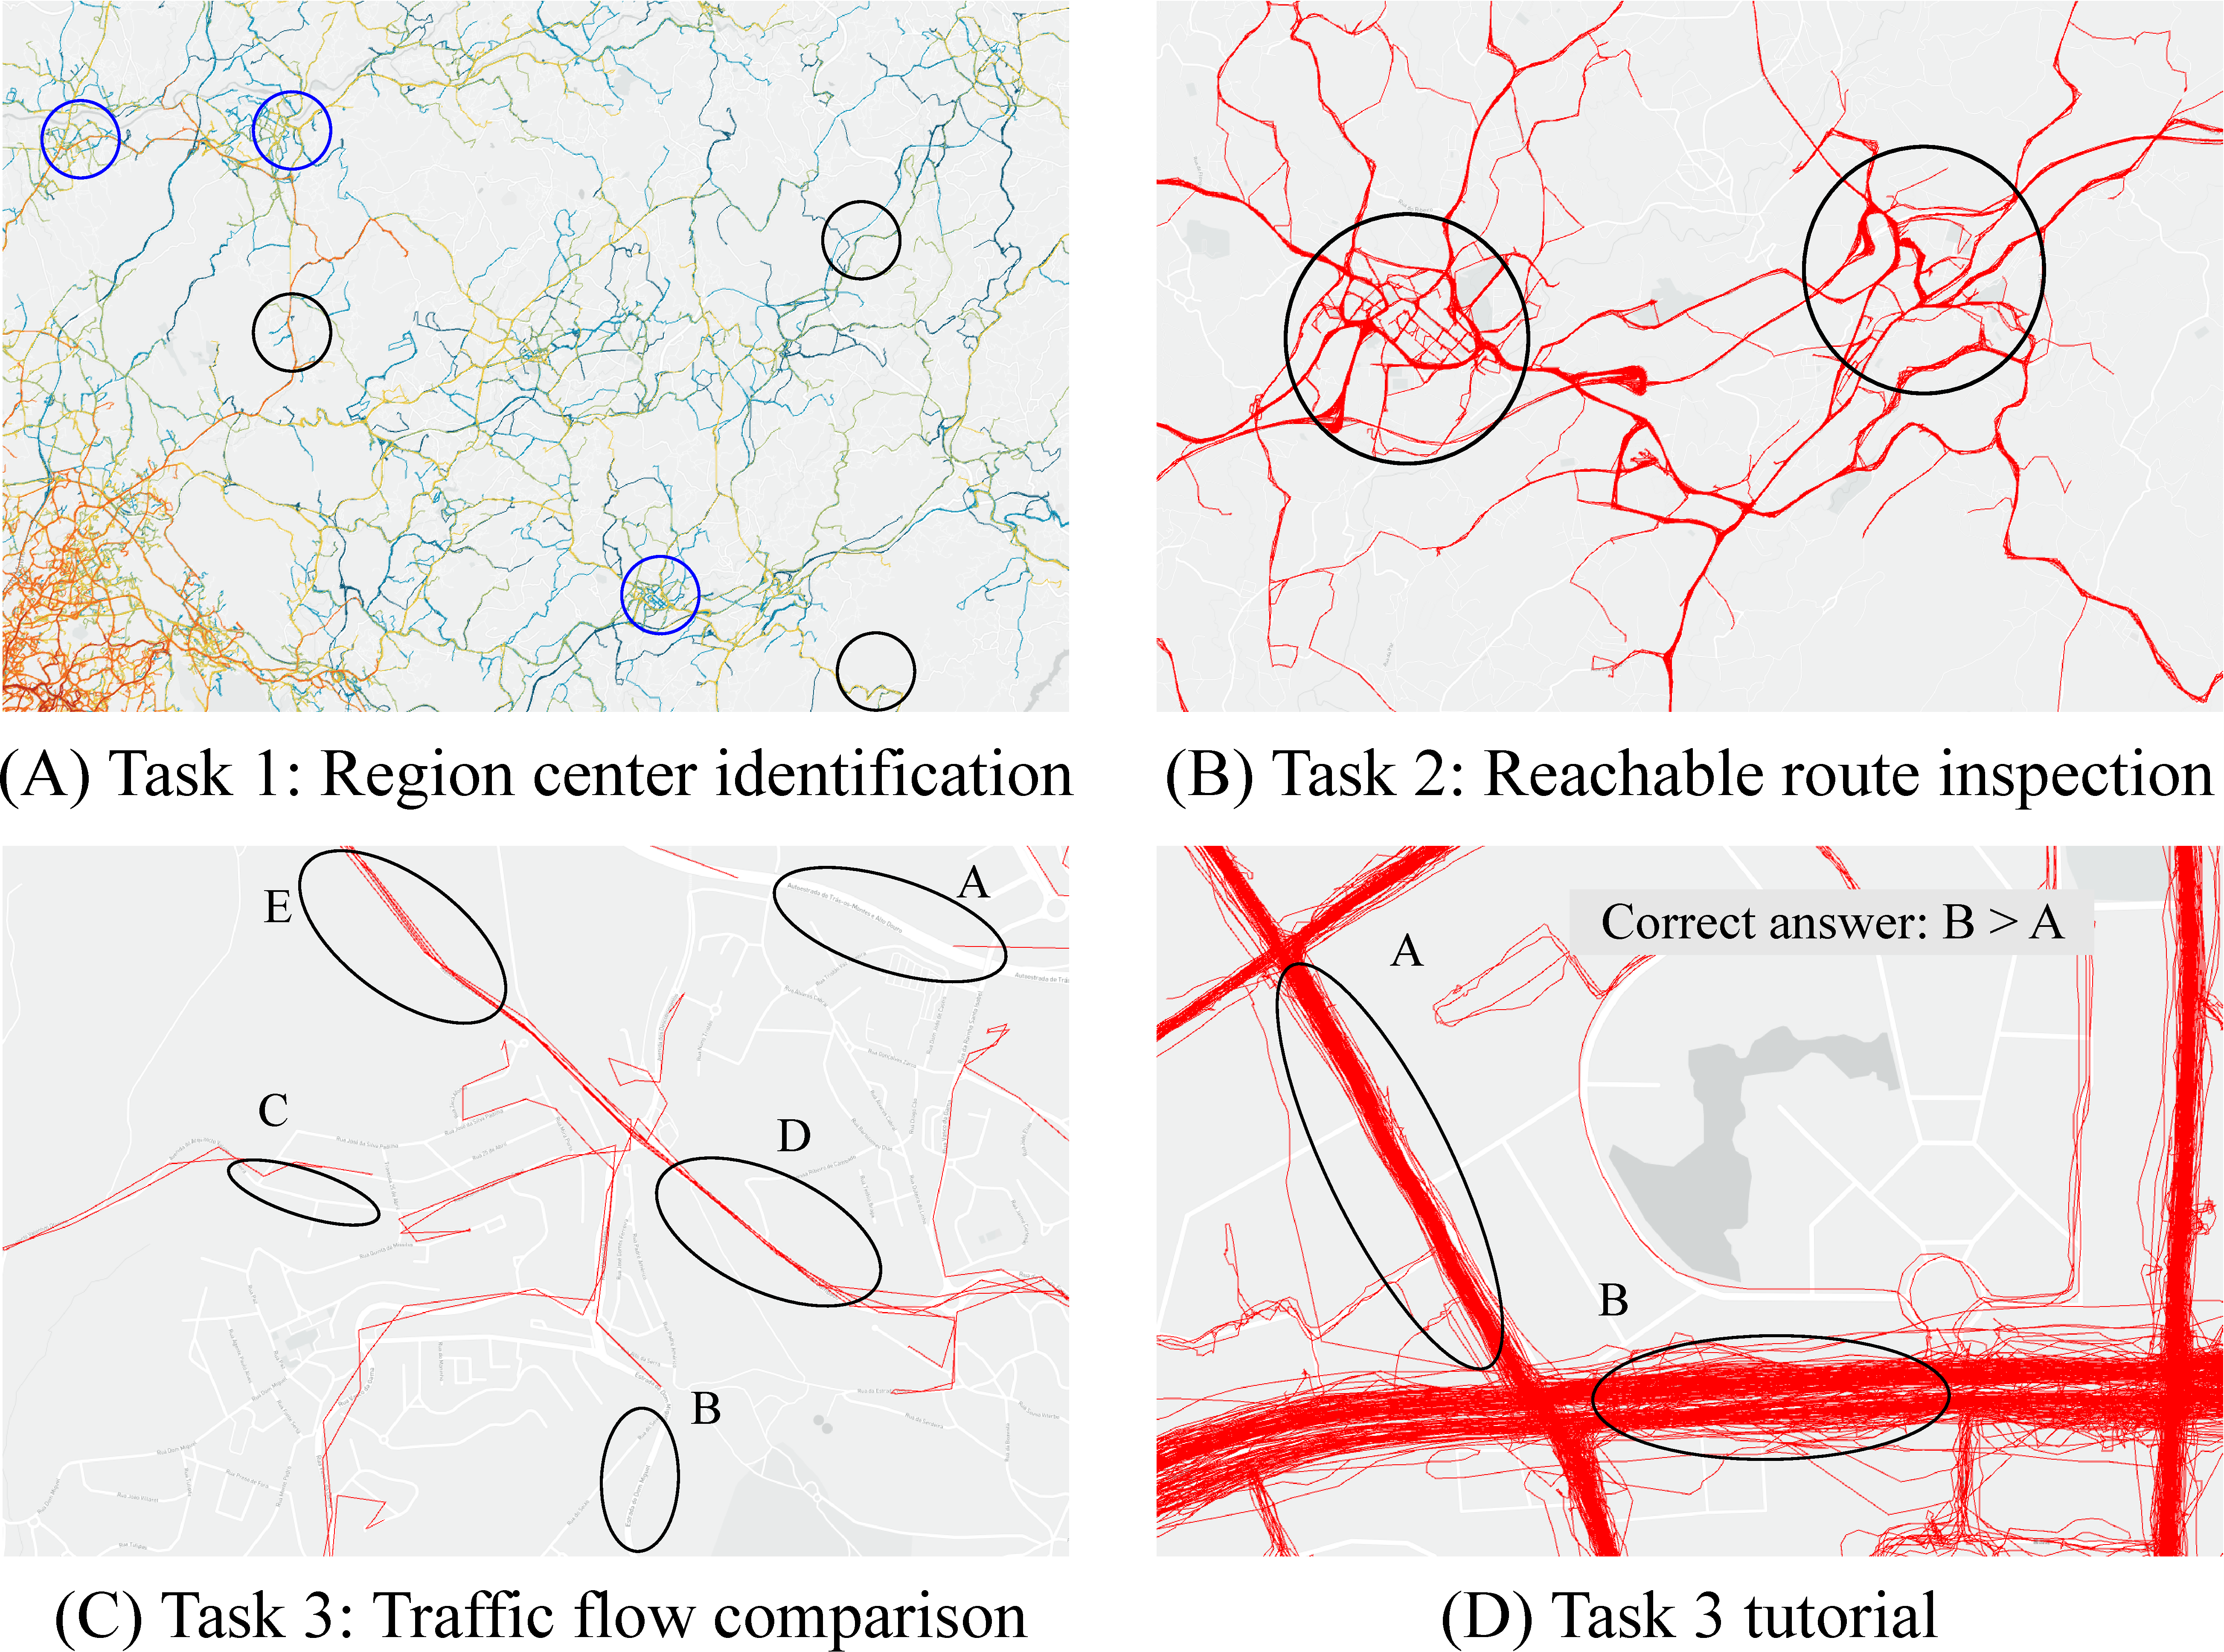
\includegraphics[width=0.45\textwidth]{pictures/user_study/interface.pdf}
	\vspace{-3mm}
	\caption{The three tasks in the user study.}
	\label{fig:apps}
	\vspace{-4mm}
\end{figure}

%\subsubsection{Settings}\label{sec:uset}

\stitle{Settings}
We recruited 186 participants with 24 females, 162 males, aged 18-29 with a mean of 21.16 for the user study\footnote{We are aware of the gender and age bias in the participants as we mainly recruited students from a university due to some practical constraints. However, we think the test results are still informative as we observed that the performance of a participant in the tasks is not significantly affected by these factors.}. The user study system is a web-based platform, in which all visualizations are displayed with a resolution of 450*300. We used the two taxi trajectory datasets, i.e., \pt{} and \sz{}, to generate the visualizations.


We test five visualization methods: (i) exact visualization using the full dataset, denoted as $\full$; (ii) uniform random sampling, denoted as $\rand$; (iii) our $\vats$ algorithm; (iv) our $\avats$ algorithm; (v) $\avats$ with color encoding, denoted as $\cavats$. The sampling rate is $\alpha = 0.5\%$ for $\rand$ and our algorithms, and $\delta = 64$ for $\avats$ and $\cavats$. The tasks are described as follows:


\textit{(T1): region center identification.} The downtown areas or commercial regions of a city are hubs for human activities and crucial for traffic management. We also observed that the taxi trajectories are denser in these regions than the other regions for both datasets. T1 contains 30 visualizations of six selected regions, which include city or commercial centers from the \pt{} dataset. For each visualization, we manually label three locations as region centers, and randomly generate three locations far away from the correct centers as fake centers. Each participant is asked to check six randomly selected visualizations and choose three region centers from each visualization, as illustrated in Figure~\ref{fig:apps}(A).

%We are interested in the average user accuracy under different visualization methods.


\textit{(T2): reachable route inspection.} Visualized trajectories should show reachable routes that connect different regions and allow users to identify them. In this task, a participant is presented with a visualization containing two circular areas (as shown in Figure~\ref{fig:apps}(B)) and asked to draw the representative reachable routes between the two areas. We assume that a route is more representative if there are a larger number of trajectories containing it. For each visualization, we manually generate at least 5 reachable routes and a user answer is considered correct if it contains 3 of these routes. T2 includes 35 visualizations of seven different regions, and for each visualization, two cities/commercial districts are marked by circles. Each participant is asked to check five randomly selected visualizations.


\textit{(T3): traffic flow comparison.} A road with a large traffic flow (i.e., having many trajectories passing it) should have dense and broad trajectory brunch in the visualization. For the $\avats$ algorithm with color encoding, such large track flow can also be identified by the concentration of trajectories with darker colors. In this task, we ask the participants to choose the road with larger traffic flow from two roads according to the visualization results, as shown in Figure~\ref{fig:apps}(C). They can also choose ``I am not sure'' if they could not decide the answer. T3 includes the visualizations of five randomly selected regions, 25 visualization results, and 60 comparison road pairs. We count the exact number of passing trajectories for each road to deduce the ground-truth answer.




%\textbf{T1. City/commercial region center identification.}
%% what participants do
%As shown by Figure~\ref{fig:user_study}(C), a visualization view was given and several regions were marked by circle. The participants needed to select the regions which could be city/commercial centers by click the corresponding circles. In each task, the number of correct regions were given.
%%Why possible
%The city or commercial region centers always have more passing trajectories from different directions than the surrounding regions, which results in the \UC{start-shape} cluster of trajectories in the visualization.
%%Generate the data
%To generate the test data of T1, we randomly chose several visualization views which contain city/commercial regions and labeled the locations of each city/commercial region center on the visualization as the correct locations first.  Then we randomly generated locations and remove the locations close to the correct locations, the remaining locations are the error locations. In each task of T1, with a given visualization, the same number of correct and wrong locations will be randomly selected.
%
%\textbf{T2. Reachable route inspection.}
%% what participants do
%Figure~\ref{fig:user_study}(D) shows the interface of T2, which includes a visualization and two circular regions. The users needed to draw several most representative reachable routes to connect the two regions. The number of the reachable routes is given.
%%Why possible
%The reachable routes indicate the routes connecting two regions, these routes must have the passing trajectories.
%%Generate the data
%To generate the test data, we randomly chose the visualization views which contain two or more city/commercial regions. In each task of T2, a visualization and two regions were randomly selected.

%\textbf{T3. Traffic flow estimation}.
%% what participants do
%As shown by Figure~\ref{fig:user_study}(B), with a given visualization, some road segments will be identified by ellipses(shown as~\ref{fig:user_study}(B)). Several road segment pairs were randomly selected and listed below the view. The participants were asked to choose the one with larger traffic flow by clicking the radio box. They can also choose ``I am not sure'' if they cannot decided the answer.
%%Why possible
%
%%Generate the data
%To generate the test data of T3,  we sampled and selected the visualization views which contain clear road structures. Then the number of trajectories passing through each road segment was counted as the traffic flow.



\stitle{User study procedure}
When the participants enter the user study system, they are first given a brief introduction about the motivation of the study and the tasks. For each tasks, we include a tutorial (with the correct result) to help the participants to get familiar with the interface and tasks. For example, Figure~\ref{fig:apps}(D) shows a tutorial for T3, where road B has larger traffic flow than road A and the correct answer is displayed on upper right corner. For each participant and task, we randomly choose visualizations and question instances from our task base. The participants are interviewed to collect feedbacks after finishing the test and their answers are saved for result analysis. We are mainly interested in how different visualization methods affect the accuracy in processing the three tasks. The readers can refer to our supplementary video for more details about our user study tasks and procedures.


%To evaluate the answers given by the participants, we refer the reviewers to our supplementary video for details of our user study procedure.

%The user study began with the introduction which introduces the motivation, tasks and visual encoding.
%Then the following sessions are divided into three blocks according to the task types. Each block starts with a task tutorial, in which the participants could perform several demo tasks, thus familiarizing themselves with the interface, interaction and tasks. For example, Figure~\ref{fig:user_study}(A) shows the demo task of T3, in which the users can check the correct answer after clicking the ``check'' button. After all the questions are finished, the answers and time usage are collected and saved in the database for the further analysis.

\stitle{Result analysis}
%\TB{Figure~\ref{fig:accuracy} depicts the average accuracy of the different visualization approaches on different tasks from all user study participates.
%Given a task with specified approach, we visualize the average accuracy of all questions by a colored circle and a line-segment to indicate the highest and lowest score of all questions of this task.}
Figure~\ref{fig:accuracy} reports the average accuracy of the five visualization methods in the three tasks.


%\begin{figure}[t]
%	\centering
%	\includegraphics[width=0.40\textwidth]{pictures/user_study/accuracy.png}
%	\vspace{-4mm}
%	\caption{Average accuracy of three types of tasks. X axis indicates the task types. Y axis indicates the accuracy of different approaches.}
%	\label{fig:accuracy}
%	\vspace{-6mm}
%\end{figure}

\begin{figure}[t]
	\centering
	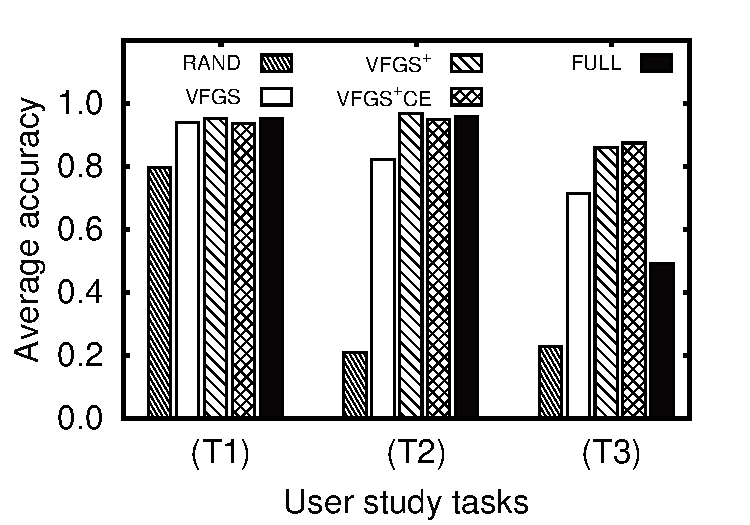
\includegraphics[width=0.3\textwidth]{pictures/userstudy}
	\vspace{-3mm}
	\caption{Average accuracy of the three tasks. X-axis shows different tasks while Y-axis indicates the accuracy.}
	\label{fig:accuracy}
	\vspace{-6mm}
\end{figure}

For (T1) region center identification, the accuracies of our proposals are very similar to that of visualizing the full dataset (i.e., $\full$). In contrast, the accuracy of $\rand{}$ is significantly lower than $\full$. These results suggest that our proposals successfully preserve the centers of human activities even with a low sampling rate of $0.5\%$. $\cavats$ performs slightly worse than $\avats$ and $\full$, and some participants reported that the colors of the trajectories distract them in the post-interview.


%the participants using all the three proposed methods had a very close performance with the participants using whole dataset, indicating the proposed methods can replace the whole dataset with a guaranteed performance in the exploration of human activity center with trajectory visualization.

For (T2) reachable route inspection, $\rand$ has a very low accuracy compared with the other 4 visualization methods. This is because $\rand$ lost many fine-grained details of the trajectories due to uniform sampling, especially in the sparse regions. However, these details can be crucial for determining the existences of a route. Moreover, our advanced methods $\avats$ and $\cavats$ provide noticeably better performance than $\vats$. This is because $\avats$ and $\cavats$ take data distribution and human perception intro consideration, and sample more trajectories in the sparse regions. As a result, more details are preserved.
%It also is worth to point out our $\avats$ (with average accuracy 0.968) outperforms the visualizations of $\full$ (with average accuracy 0.959) slightly.

%Interestingly,
%For the tasks of T2, $\avats$, $\avats$ with color encoding and the whole dataset all have similar accuracy scores which are far higher than random sampling.
%Moreover, $\avats$ and $\avats$ with color encoding also outperforms the $\vats$ clearly by taking the perception parameters into consideration.
% This results demonstrate the advantage of $\avats$ on the urban exploration at a detail level.

(T3) traffic flow comparison is more difficult than T1 and T2, and thus the accuracy drops for all visualization methods. Similar to the case of T1 and T2, $\rand$ has the worst performance among all methods. Remarkably, the accuracies of our proposals (i.e.,  $\vats,\avats$ and $\cavats$) are even higher than $\full$. In the post-interview, the participants reported that $\full$ has severe visual clutter problem, which makes it difficult to compare the traffic flows on two roads. Therefore, the higher accuracies of our proposals indicate that sampling effectively mitigates visual clutter. In addition, the accuracies of $\avats$ and $\cavats$ are higher than that of $\vats$, suggesting that our advanced method and color encoding are effective in alleviating visual clutter.

To sum up, the results in this part shows that our proposals (i.e., ($\vats$, $\avats$, and $\cavats$) are effective in practical spatial tasks. All our methods consistently outperforms $\rand$ by a large margin across different tasks, the advanced methods (i.e., $\avats$, and $\cavats$) often achieve comparable or even better performance than  $\full$.

%\vspace{-2mm}
\subsection{Quantitative Evaluation}\label{sec:quality}
In this part, we quantitatively evaluates our proposals on the \pt{} and \sz{} trajectory datasets from two aspects:
(i) visual fidelity at different zoom levels
and (ii) running time under different sampling rates.

\begin{figure}
 \centering
 \small
 \begin{tabular}{cc}
   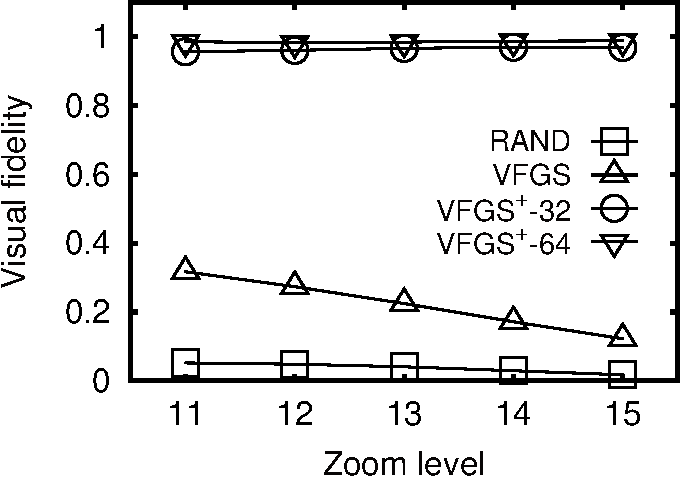
\includegraphics[width=0.44\columnwidth]{pictures/fporto}
   &
   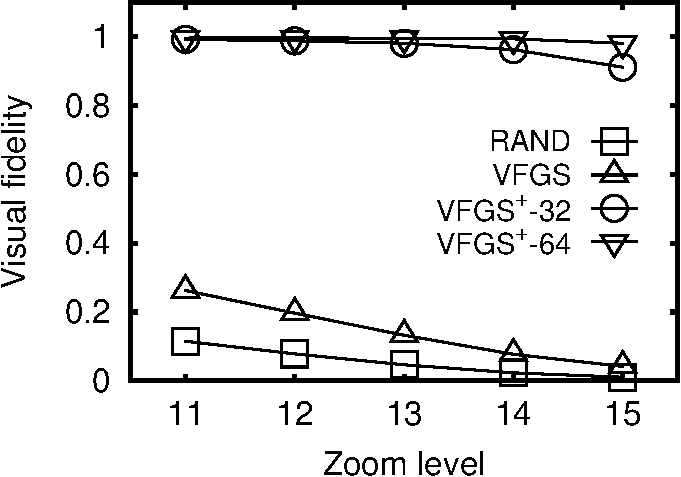
\includegraphics[width=0.44\columnwidth]{pictures/fshenzhen}
   \\
   (A) \pt{}
   &
   (B) \sz{}
 \end{tabular}
 \vspace{-3mm}
 \caption{Visual fidelity vs. zoom levels.}
 \label{fig:fidelity}
 \vspace{-3mm}
\end{figure}

\stitle{Visual fidelity evaluation} We report the \textit{visual fidelity} of different visualization methods in Figure~\ref{fig:fidelity}. Visual fidelity is defined as the $1-loss$, in which $loss$ is the fidelity loss function in Equation~\eqref{eqref:loss}. The sampling rate is $\alpha=0.5\%$ and the visualization using the full dataset is used as the ground-truth. The results show that $\rand$ always has the lowest  visual fidelity. $\vats$ has better visual fidelity than $\rand$ but is significantly outperformed by $\avats$. With $\delta=32$ and $\delta=64$, the minimum visual fidelity values of $\avats$ are 0.95 and 0.91 for \pt{} and \sz{}, respectively. Moreover, the fidelity of all methods increases when the zoom level drops, which in line with Theorem~\ref{the:level}.


%We first evaluate the visual fidelity of our proposed methods.
%We measure the visual fidelity of different approaches over the $\full$ by using the $loss()$ function defined in Section~\ref{sec:def}.
%Figure~\ref{fig:fidelity}(A) and (B) show the visual fidelity of $\rand$, $\vats$, $\avats$ with $\delta=32$ and $\avats$ with $\delta=64$ from zoom level 11 to 15 (i.e., overview to detail view) in
%\pt{} and \sz{}, respectively.
%Results show that $\rand$ does not guarantee the visual fidelity of the result.
%Although $\vats$ offers theoretical visual fidelity guarantee w.r.t. the optimal sampled result set with a given sampling rate, it still has room for improvement over the $\full$;
%Moreover, $\avats$ with $\delta=32$ and $\delta=64$ has excellent visual fidelity w.r.t. the $\full$ dataset. The minimum visual fidelity value is 0.95 and 0.91 in \pt{} and \sz{}, respectively.
%It also confirms the superiority of our proposal.
%The visual fidelity of $\avats$ falls with the rising of zoom levels, e.g., from zoom level 11 to 15.
%The reason is the higher zoom level, the more details are expected.


\begin{figure}
 \centering
 \small
 \begin{tabular}{cc}
   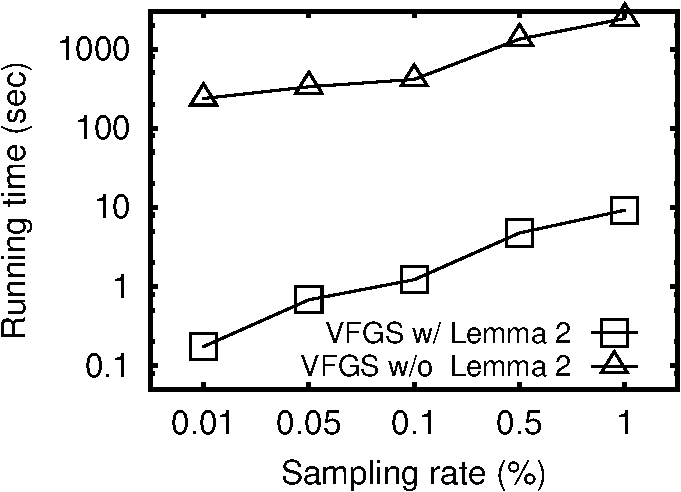
\includegraphics[width=0.44\columnwidth]{pictures/tporto}
   &
   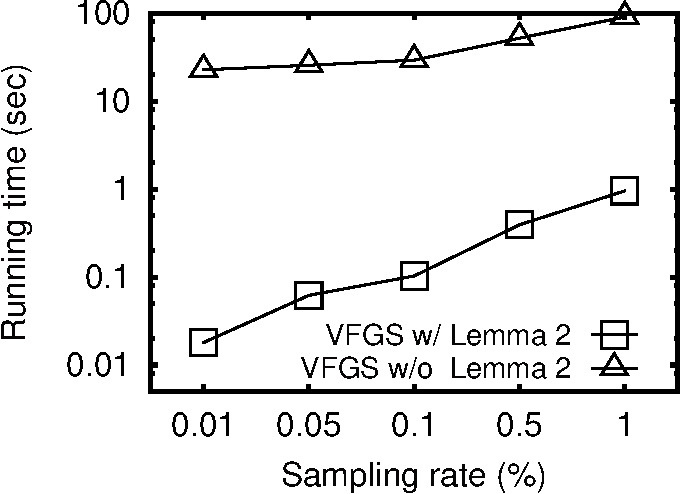
\includegraphics[width=0.44\columnwidth]{pictures/tshenzhen}
   \\
   (A) \pt{}
   &
   (B) \sz{}	
 \end{tabular}
 \vspace{-3mm}
 \caption{Running time of $\vats$ w/ and w/o Lemma~\ref{lem:submodular}.}
 \label{fig:cost}
 \vspace{-3mm}
\end{figure}


\stitle{Running time evaluation} We report the running time of our $\vats$ algorithm in Figure~\ref{fig:cost} by varying the sampling rate from $0.01\%$ to $1\%$. The results show that $\vats$ is quite slow without the submodularity of contribution value, which agrees with Lemma~\ref{lem:submodular} in Section~\ref{sec:opt}.
The optimized $\vats$ (e.g., $\vats$ with Lemma~\ref{lem:submodular}) outperforms $\vats$ by one to three orders of magnitudes on both datasets. The result show that running time of our $\vats$ algorithm is below 1 second in most cases. We have shown that $\vats$ provides good visualization performance with a low sampling rate (e.g., $0.1\%$ or $1\%$) in Section 6.1 and 6.2, and our technical report suggests that the rendering latency scales almost linearly with dataset cardinality. By significantly reducing the dataset cardinality with sampling, $\vats$ can effectively reduces the rendering latency to make interactive visualization possible without sacrificing visual fidelity. For example, rendering the full $\pt{}$ dataset takes about 34 seconds, with a sampling rate of $1\%$, $\vats$ can bring down the rendering latency to less than 1 second.







\section{Conclusions and future directions}\label{sec:con}
%Visualizing large trajectory dataset is challenge due to two reasons: visual clutter and long rendering time.
%Data sampling technique, an effective method in reducing the rendering time by shrinking the data size, has been applied in a variety of data.
%However, very few work target at the trajectory sampling especially from the perspective of visualization.
%The most commonly used sampling method, uniform random sampling technique, always generate results with very poor visual quality because very few trajectories located at margin regions can be preserved.
%We fill the gap by proposing a novel sampling techniques $\avats$ which guarantees the visual quality at overview and reduce the visual clutter at the detail view. The technique characteristics and a series of parameters setting are discussed.
%We compare $\avats$ with uniform random sampling in regarding to visual quality preservation and time-usage. We evaluate the effectiveness of proposed method by applying our method to different dataset and conducting users studies on specific interactive trajectory exploration tasks.
%Even though it is recommended to use our method with caching techniques, our experience in the experiment shows that a faster algorithm will be more user friendly for the real world ad-hoc exploration tasks. For future work, we first plan to reduce the time usage by leveraging the advanced database techniques such as the indexing technique or use GPU acceleration.
%In addition, there are several directions can be further explored to enrich the information presented by the visualization.
%First we will develop different color encoding schema to present the spatial distribution of trajectory more precisely.
%In current schema, the color of one trajectory is the same, thus the color of the long trajectories may mislead the users because they pass  through many regions with different level of the traffic crowdedness. One solution is to use gradient color schema to encode the trajectories.
%Another interesting direction is to extend the approach to support the mulit-class characteristics which is a commonly existed in variety of trajectory dataset.
This paper presents a novel sampling technique, $\avats$, that guarantees the visual fidelity of line-based trajectory visualization and alleviates the visual clutter problem. The effectiveness and efficiency of the proposed method are validated with real world visual analysis tasks and quantitatively performance measurements. Possible future directions include (i) improving visual fidelity by sampling trajectory segments instead of complete trajectories and (ii) developing advanced color encoding schemes to better describe the spatial distribution of the trajectories.
%extending our approaches to support the specific trajectory features such as mulit-class characteristics.

%we focus on the sampling approach of trajectory segments other than the whole trajectories to achieve higher visual fidelity.
%We will also develop different color encoding schema to present the spatial distribution of trajectories more precisely. Currently, the color of one trajectory keep the same, thus the color of the long trajectories may mislead the users because they may pass through many regions with different traffic crowdedness.
%We also consider to extend our approach to support the specific trajectory features such as mulit-class characteristics. 



%\begin{acks}
% This work was supported by the [...] Research Fund of [...] (Number [...]). Additional funding was provided by [...] and [...]. We also thank [...] for contributing [...].
%\end{acks}


\bibliographystyle{ACM-Reference-Format}
\bibliography{ref}

\end{document}
\endinput
